
\documentclass[oneside,a4paper,14pt]{extreport}
%\documentclass{article}


% Font tiếng Việt
\usepackage[T5]{fontenc}
\usepackage[utf8]{inputenc}
\DeclareTextSymbolDefault{\DH}{T1}

% Tài liệu tham khảo
\usepackage[
	sorting=nty,
	backend=bibtex,
	defernumbers=true]{biblatex}
\usepackage[unicode]{hyperref} % Bookmark tiếng Việt
\addbibresource{References/references.bib}

\makeatletter
\def\blx@maxline{77}
\makeatother

% Chèn hình, các hình trong luận văn được để trong thư mục Images/
\usepackage{graphicx}
\graphicspath{ {Images/} }

%không biết dòng gì nữa
\usepackage[usenames,dvipsnames]{xcolor}
\PassOptionsToPackage{usenames,dvipsnames}{xcolor}
\PassOptionsToClass{aspectratio=169}{beamer}

% Chèn và định dạng mã nguồn


\usepackage{listings}
\usepackage{color}
\definecolor{codegreen}{rgb}{0,0.6,0}
\definecolor{codegray}{rgb}{0.5,0.5,0.5}
\definecolor{codepurple}{rgb}{0.58,0,0.82}
\definecolor{backcolour}{rgb}{0.95,0.95,0.92}
\lstdefinestyle{mystyle}{
    backgroundcolor=\color{backcolour},   
    commentstyle=\color{codegreen},
    keywordstyle=\color{magenta},
    numberstyle=\tiny\color{codegray},
    stringstyle=\color{codepurple},
    basicstyle=\footnotesize,
    breakatwhitespace=false,         
    breaklines=true,                 
    captionpos=b,                    
    keepspaces=true,                 
    numbers=left,                    
    numbersep=5pt,                  
    showspaces=false,                
    showstringspaces=false,
    showtabs=false,                  
    inputencoding=utf8,
    tabsize=2
}
\lstset{style=mystyle}

% Chèn và định dạng mã giả
\usepackage{amsmath}
\usepackage{algorithm}
\usepackage[noend]{algpseudocode}
\makeatletter
\def\BState{\State\hskip-\ALG@thistlm}
\makeatother

\usepackage[utf8]{inputenc}
%\usepackage{minted}

% Bảng biểu
\usepackage{multirow}
\usepackage{array}
\newcolumntype{L}[1]{>{\raggedright\let\newline\\\arraybackslash\hspace{0pt}}m{#1}}
\newcolumntype{C}[1]{>{\centering\let\newline\\\arraybackslash\hspace{0pt}}m{#1}}
\newcolumntype{R}[1]{>{\raggedleft\let\newline\\\arraybackslash\hspace{0pt}}m{#1}}



 
% Đổi tên mặc định
\renewcommand{\chaptername}{Chương}
\renewcommand{\figurename}{Hình}
\renewcommand{\tablename}{Bảng}
\renewcommand{\contentsname}{Mục lục}
\renewcommand{\listfigurename}{Danh sách hình}
\renewcommand{\listtablename}{Danh sách bảng}
\renewcommand{\appendixname}{Phụ lục}

% Định dạng chapter
\usepackage{titlesec}
\titleformat{\chapter}
    [display] 
    {\normalfont\bfseries\Large}{\chaptername \ \thechapter}{10pt}{\huge}
\titlespacing*{\chapter}{0pt}{-10pt}{40pt} %khoảng cách giữa chapter và đầu trang

\titleformat{\section}
    {\normalfont\bfseries\large}{\thesection}{1em}{}
 
\titleformat{\subsection}
    {\normalfont\bfseries\normalsize}{\thesubsection}{1em}{}
  
% Dãn dòng 1.5
\usepackage{setspace}
\onehalfspacing

% Thụt vào đầu dòng
\usepackage{indentfirst}

% Canh lề
\usepackage[
  top=20mm,
  bottom=10mm,
  left=30mm,
  right=20mm,
  footskip = 15mm,
  includefoot]{geometry}
  
% Trang bìa
\usepackage{tikz}
\usetikzlibrary{calc}
\newcommand\HRule{\rule{\textwidth}{1pt}}

% ========================================================================================= %
% CHÚ Ý: Thông tin chung về KLTN - sinh viên điền vào đây để tự động update các trang khác  %
% ========================================================================================= %
\newcommand{\tenSV}{Nguyễn~Khôi~Nguyên~-~Nguyễn~Tuấn~Phùng~-~Hồ~Bùi~Văn~Quang} % Dấu ~ là khoảng trắng không được tách (các chữ nối với nhau bằng dấu ~ sẽ nằm cùng 1 dòng
\newcommand{\mssv}{1753087~1753087~1753093}
\newcommand{\tenKL}{Xây~dựng~hệ~thống~hỏi~đáp~pháp~luật} % Chú ý dấu ~ trong tên khóa luận
\newcommand{\tenGVHD}{Nguyễn~Trường~Sơn~-~Nguyễn~Thị~Như~Anh}
\newcommand{\tenBM}{Hệ~Thống~Thông~Tin}

\begin{document}

\begin{titlepage}

\begin{center}

TRƯỜNG ĐẠI HỌC KHOA HỌC TỰ NHIÊN\\
\textbf{KHOA CÔNG NGHỆ THÔNG TIN}\\[2cm]


{ \Large \bfseries Nguyễn Khôi Nguyên\\ } 
{ \Large \bfseries Nguyễn Tuấn Phùng\\} 
{ \Large \bfseries Hồ Bùi Văn Quang\\[1cm] } 


{ \Large \bfseries ĐỒ ÁN TỐT NGHIỆP\\[3cm]} 


\large ĐỒ ÁN TỐT NGHIỆP CỬ NHÂN\\


\large CHƯƠNG TRÌNH CHẤT LƯỢNG CAO\\


\begin{tikzpicture}[remember picture, overlay]
  \draw[line width = 2pt] ($(current page.north west) + (2cm,-2cm)$) rectangle ($(current page.south east) + (-1.5cm,2cm)$);
\end{tikzpicture}

\vfill
Tp. Hồ Chí Minh, tháng 08/2021

\end{center}

\pagebreak



\begin{center}

TRƯỜNG ĐẠI HỌC KHOA HỌC TỰ NHIÊN\\
\textbf{KHOA CÔNG NGHỆ THÔNG TIN}\\[2cm]


{\large \bfseries Nguyễn Khôi Nguyên - 1753078\\} 
{\large \bfseries Nguyễn Tuấn Phùng - 1753087\\} 
{\large \bfseries Hồ Bùi Văn Quang - 1753093\\[2cm]}

%Tên đề tài Khóa luận tốt nghiệp/Đồ án tốt nghiệp

{ \Large \bfseries XÂY DỰNG HỆ THỐNG HỎI ĐÁP PHÁP LUẬT VIỆT NAM\\ĐỒ ÁN TỐT NGHIỆP\\[1cm] } 




\large ĐỒ ÁN TỐT NGHIỆP CỬ NHÂN\\

\large CHƯƠNG TRÌNH CHẤT LƯỢNG CAO\\[1cm]


\textbf{GIÁO VIÊN HƯỚNG DẪN}\\
TS. Nguyễn Trường Sơn\\
ThS. Nguyễn Thị Như Anh

\begin{tikzpicture}[remember picture, overlay]
  \draw[line width = 2pt] ($(current page.north west) + (2cm,-2cm)$) rectangle ($(current page.south east) + (-1.5cm,2cm)$);
\end{tikzpicture}

\vfill
Tp. Hồ Chí Minh, tháng 08/2021

\end{center}

\end{titlepage}
% Sasu trang Title, các bạn chèn nhận xét gủa GVHD và GVPB. Nhận xét sẽ được giáo vụ phát sau buổi bảo vệ để các bạn đóng quyển.

%\pagenumbering{arabic} % Đánh số i, ii, iii, ...

%\addcontentsline{toc}{chapter}{Lời cam đoan}
%\include{Appendix/reassurances}

\addcontentsline{toc}{chapter}{Lời cảm ơn}
\chapter*{\centering Lời cảm ơn}
\label{thanks}

Trong suốt thời gian học tập và rèn luyện tại Trường Đại học Khoa Học Tự Nhiên cho đến nay, chúng em đã nhận được rất nhiều sự quan tâm, giúp đỡ của quý Thầy Cô và bạn bè. Với lòng biết ơn sâu sắc và chân thành nhất, chúng em xin gửi đến Thầy Cô ở Khoa Công nghệ thông tin đã cùng với tri thức và tâm huyết của mình để truyền đạt vốnk iến thức quý báu cho chúng em trong suốt thời gian học tập tại trường.

Và đặc biệt, trong học kỳ này, Khoa đã tạo cơ hội cho chúng em được tiếp cận với Đồ án tốt nghiệp mà theo chúng em là rất hữu ích đối với chúng em cũng như tất cả các sinh viên thuộc các chuyên ngầnh Hệ Thống Thông Tin. Đó là đề tài "Áp dụng máy học vàot trong hệ thống hỏi đáp pháp luật". Chúng em xin chân thành cảm ơn thầy Nguyễn Trường Sơn và cô Nguyễn Thị Như Anh đã tận tâm hướng dẫn chúng em qua từng buổi thảo luận về nghiệp vụ cũng như kiến thức bổ sung về chuyên ngành.

Chúng em xin bày tỏ lòng biết ơn đến ban lãnh đạo của Trường Đại Học Khoa Học Tự Nhiên và các Khoa Phòng ban chức năng đã trực tiếp và gián tiếp giúp đỡ em trong suốt quá trình học tập và thực hiện đề tài này.

Với điều kiện thời gian cũng như kinh nghiệm còn hạn chế của một sinh viên, bài báo cáo này không thể tránh khỏi những thiếu sót. Chúng em rất mong nhận được sự chỉ bảo, đóng góp ý kiến của các quý thầy cô để chúng em có điều kiện bổ sung, nâng cao kiến thức của mình, phụ vụ tốt hơn công việc thực tế sau này.

Cuối cùng chúng em kính chúc quý thầy, cô dồi dào sức khoẻ và thành công trong sự nghiệp cao quý. Chúng em xin chân thành cảm ơn!

\begin{flushright}
	Nhóm thực hiện
\end{flushright}7

\addcontentsline{toc}{chapter}{Nhận xét của giáo viên hướng dẫn}
\chapter*{NHẬN XÉT CỦA GIÁO VIÊN HƯỚNG DẪN}
\label{nhanxetgiaovienhuongdan}
%	\textbf{NHẬN XÉT CỦA GIÁO VIÊN HƯỚNG DẪN}\\[1cm]
\begin{tikzpicture}[remember picture, overlay]
	\draw[line width = 2pt] ($(current page.north west) + (2cm,-2cm)$) rectangle ($(current page.south east) + (-1.5cm,2cm)$);
\end{tikzpicture}
\begin{center}
{
	\dotfill\\[0.5cm]	\dotfill\\[0.5cm]	\dotfill\\[0.5cm]	\dotfill\\[0.5cm]
	\dotfill\\[0.5cm]	\dotfill\\[0.5cm]	\dotfill\\[0.5cm]	\dotfill\\[0.5cm]	\dotfill\\[0.5cm]	\dotfill\\[0.5cm]	\dotfill\\[0.5cm]	\dotfill\\[0.5cm]
}
\end{center}

	Đồ án đáp ứng yêu cầu của Đồ án tốt nghiệp cử nhân CNTT.

\begin{flushright}
	\begin{tabular}{@{}c@{}}
	Tp.HCM, ngày ..... tháng ...... năm 2021\\
	Giáo viên hướng dẫn
	\end{tabular}
\end{flushright}

\addcontentsline{toc}{chapter}{Nhận xét của giáo viên phản biện}

\begin{titlepage}
	
	\begin{center}
		\textbf{NHẬN XÉT CỦA GIÁO VIÊN PHẢN BIỆN}\\[1cm]
		\begin{tikzpicture}[remember picture, overlay]
			\draw[line width = 2pt] ($(current page.north west) + (2cm,-2cm)$) rectangle ($(current page.south east) + (-1.5cm,2cm)$);
		\end{tikzpicture}
		{	\dotfill\\[0.5cm]	\dotfill\\[0.5cm]	\dotfill\\[0.5cm]	\dotfill\\[0.5cm]
			\dotfill\\[0.5cm]	\dotfill\\[0.5cm]	\dotfill\\[0.5cm]	\dotfill\\[0.5cm]	\dotfill\\[0.5cm]	\dotfill\\[0.5cm]	\dotfill\\[0.5cm]	\dotfill\\[0.5cm]
			\dotfill\\[0.5cm]	\dotfill\\[0.5cm]	\dotfill\\[0.5cm]
		}
		
		
		Đồ án đáp ứng yêu cầu của Đồ án tốt nghiệp cử nhân CNTT.
		
		\begin{flushright}
			\begin{tabular}{@{}c@{}}
				Tp.HCM, ngày ..... tháng ...... năm 2021\\
				Giáo viên phản biện
			\end{tabular}
		\end{flushright}
		
	\end{center}
	
\end{titlepage}



\addcontentsline{toc}{chapter}{Đề cương chi tiết}
\begin{titlepage}	
\textbf{ĐỀ CƯƠNG CHI TIẾT ĐỒ ÁN}\\[1cm]
\label{Decuongchitiet}

	\textbf{Tên đề tài:}\\
	 Xây dựng hệ thống hỏi đáp Pháp Luật  \\ 
	 
	\textbf{Giáo viên hướng dẫn:} \\
	TS. Nguyễn Trường Sơn - ThS. Nguyễn Thị Như Anh\\ 
	
	\textbf{Thời gian thực hiện:}\\
	Từ ngày 07/01/2021 đến ngày 29/07/2021      \\ 
	
	\textbf{Sinh viên thực hiện:}\\
			Nguyễn Khôi Nguyên (1753078)\\  
			Nguyễn Tuấn Phùng (1753087) \\ 
			Hồ Bùi Văn Quang (1753093)\\
			
	\textbf{Loại đề tài: }Nghiên cứu có ứng dụng demo\\ 
	
	\textbf{Kế hoạch thực hiện:}\\
	\begin{itemize}
		\item[-] \textbf{Từ 07/01 - 01/03:} Tìm hiểu về đề tài, mô hình Bert.
		\item[-] \textbf{Từ  02/03 - 01/04:} Thu thập dữ liệu từ Thư viện pháp luật, áp dụng tách từ underthesea vào bộ dữ liệu, xây dựng hệ thống sử dụng pre-trained model, xây dựng Front-end hệ thống.
		\item[-] \textbf{Từ 02/04 - 02/06:} Thay đổi phương pháp tách từ bằng sử dụng python vietnamese toolkit, xây dựng thành công được hệ thống sử dụng pre-trained model SimCSE PhoBERT.
		\item[-] \textbf{Từ 03/06 - 24/07:} Xây dựng model trên dữ liệu Pháp luật gán nhãn thủ công, chỉnh sửa giao diện Front-end,khảo sát về tình hình hỏi đáp pháp luật hiện nay, viết cuốn báo cáo.
	\end{itemize}
  \begin{minipage}{.45\linewidth}
	\begin{flushleft}
		\textbf{Xác nhận của GVHD: } 
	\end{flushleft}
\end{minipage}
\hfill
\begin{minipage}{.45\linewidth}
	\begin{flushright}
		\textbf{Sinh viên thực hiện:} 
	\end{flushright} 
\end{minipage}
\begin{flushright}
	\begin{tabular}{@{}c@{}}
		 \\[3 cm]
		
		Nguyễn Khôi Nguyên\\
		Nguyễn Tuấn Phùng\\
		Hồ Bùi Văn Quang\\
	\end{tabular}
\end{flushright}


\end{titlepage}

% Mục lục, danh sách hình, danh sách bảng
\addcontentsline{toc}{chapter}{Mục lục}
\tableofcontents
\listoffigures
\listoftables

\clearpage

\pagenumbering{arabic} % Đánh số 1, 2, 3, ...

% Các chương nội dung

\chapter{MỞ ĐẦU}
\label{Chapter1}
\textit{Nội dung Chương 1 giới thiệu thực trạng chung của nhu cầu tra cứu cũng như đặt ra những câu hỏi liên quan đến vấn đề pháp luật ở Việt Nam, từ đó hình thành nên lý do và mục tiêu để thực hiện đồ án.}
\section{Giới thiệu chung}
	Hiện nay, nhu cầu tìm kiếm cũng như hỏi đáp các vấn đề liên quan đến các lĩnh vực trong đời sống đang rất lớn, đặc biệt là sử dụng các dịch vụ tra cứu trực tuyến. Các lĩnh vực có nhu cầu tìm kiếm thông tin như công nghệ, chính trị, xã hội, luật pháp,.... Đặc biệt là trong lĩnh vực luật pháp, điều mà trước đây chỉ có thể sử dụng phương pháp truyền thống là đến các cơ sở có khả năng pháp lý như văn phòng luật sư, các cơ sở có quyền về pháp lý,... mà người có nhu cầu muốn giải đáp thắc mắc có thể đến và đặt ra những câu hỏi cụ thể để từ đó, những chuyên gia có thể giải đáp được những câu hỏi cho họ.
	
	Nhưng với thời điểm công nghệ 4.0 hiện nay, việc sử dụng internet đối với mỗi người chúng ta là điều thiết yếu trong cuộc sống. Vậy nên, việc xuất hiện các trang web, những dịch vụ trực tuyến nhằm giải đáp những vấn đề trên được hình thành. Tuy nhiên, có một số điểm yếu mà còn tồn tại trong hệ thống này là:
	\begin{itemize}
		\item Các câu hỏi được giải đáp bởi các chuyên gia và chỉ được lưu trữ dạng văn bản thuần.
		\item Khi cần tra cứu câu hỏi, người dùng cần phải nhập đúng chính xác câu hỏi hoặc chính xác từ khoá mà có câu hỏi mẫu đã được lưu trữ trong cơ sở dữ liệu của hệ thống.
		\item Nếu như người dùng cần tìm những câu hỏi có nội dung tương tự như câu hỏi đang cần hỏi thì cần phải biết được lĩnh vực mà câu hỏi đã được hỏi.
	\end{itemize}


\section{Mục tiêu đề tài}
Với nhu cầu trao đổi thông tin hiện nay ngày càng cao cùng với sự phát triển của mạng Internet và công nghệ, hằng ngày con người luôn phải xử lý một lượng thông tin lớn. Do đó việc hỏi đáp mang tính thiết yếu hơn trong cuộc sống, và nhiều trang web, hệ thống hỏi đáp đã được xây dựng nên để đáp ứng nhu cầu đó. Nhưng trong số đó, vẫn còn nhiều hệ thống hỏi đáp chưa thể đưa ra câu trả lời ngay lập tức được hoặc phải do chính nhân tố con người trả lời một cách thủ công. Đặc biệt khi nói về lĩnh vực Pháp luật – lĩnh vực mang tính chất khô khan và cần nhiều sự chính xác và nhanh chóng khi đưa ra câu trả lời đối với một hệ thống hỏi đáp thì hiện nay vẫn chưa có nhiều hệ thống đáp ứng được.

Đề tài hướng đến mục tiêu là xây dựng một hệ thống hỏi đáp tự động tiếng Việt cho một lĩnh vực cụ thể là về pháp luật Việt Nam. Bằng cách áp dụng công nghệ nhiều hơn, ở đây chính là công nghệ trí tuệ nhân tạo giúp nâng cao hiệu quả, tốc độ và sự chính xác trong câu trả lời mà hệ thống đưa ra. Với hướng tiếp cận xử lý ngôn ngữ tự nhiên, sử dụng các Pre-trained Model (mô hình tiền huấn luyện) để phân tích ngữ nghĩa của các câu hỏi và cho ra kết quả chính xác nhất thì việc xây dựng một hệ thống về hỏi đáp Pháp luật Việt Nam là một đề tài hoàn toàn khả thi.

\pagebreak
\section{Nội dung của đồ án}

Đồ án có tổng cộng 7 chương với nội dung chính như sau:

\textbf{Chương 1:} Mở đầu

    Nội dung chương 1 giới thiệu về thực trạng về nhu cầu trong thực tế của việc hỏi đáp các vấn đề liên quan đến luật pháp ở Việt Nam, đưa ra các điểm yếu trong phương pháp truyền thống và đưa ra mục tiêu, phương pháp áp dụng của đồ án vào trong ứng dụng.

\textbf{Chương 2:} Khảo sát hiện trạng
	Nội dung chương 2 là báo cáo từ một khảo sát nhỏ của nhóm nhằm xác định được rằng trong thực tế thì có những nhóm người dùng nào sẽ có nhu cầu tìm kiếm, hỏi đáp về pháp luật và cách thức để người dùng tìm được đáp án cho vấn đề đang cần tìm kiếm.

\textbf{Chương 3:} Công nghệ sử dụng

    Nội dung của chương 2 là đưa ra các cơ sở lý thuyết để áp dụng vào trong đề tài, chỉ ra các công nghệ được áp dụng và phối hợp với nhau để giải quyết được vấn đề cần phải giải quyết trong đề tài nghiên cứu.

\textbf{Chương 4:} Thu Thập Dữ Liệu

    Nội dung chương 3 là trình bày về tổng quan của hệ thống và quy trình để xây dựng nên hệ thống về phần Back-end và Front-end.

\textbf{Chương 5:} Kiến trúc phần Back-end
	\begin{itemize}
		\item Trình bày chi tiết về quá trình thu thập dữ liệu pháp luật
		\item Phương pháp xây dựng cơ sở dữ liệu và lưu trữ dữ liệu
		\item Mô hình đào tạo dữ liệu phương pháp phân tích đưa ra được thông tin chuẩn xác từ mô hình. 
	\end{itemize}

\textbf{Chương 6:} Kiến trúc phần Front-end

    Trình bày về trình tự và cách để đưa dữ liệu được trả về ở phần Back-end hiển thị lên giao diện người dùng.

\textbf{Chương 7:} Kết luận và hướng phát triển
    Nội dung chương 5 là tóm tắt lại kết quả đạt được sau khi hoàn thành đề tài, ý nghĩa của đề tài và định hướng phát triển của đề tài trong tương lai


\chapter{Chương 2: Khảo sát }
\label{Chapter2}

\textit{Nội dung của chương 2 trình bày về việc khảo sát thực tế người dùng mạng internet phổ thông có nhu cầu hoặc có kinh nghiệm về việc tra cứu thông tin, hỏi đáp các vấn đề về pháp luật ở Việt Nam. }

\section{Khảo sát}
Nhằm thu thập ý kiến, tìm hiểu hiện trạng của nhu cầu cần tìm hiểu về Pháp luật của người dùng, nhóm đã thực hiện một cuộc khảo sát trực tuyến của người dùng internet bao gồm người đi làm và cả những sinh viên của các trường đại học trong nước. Nội dung câu hỏi như sau:

\begin{itemize}
	\item Bạn hiện là sinh viên hay đang đi làm?
	\item Bạn hoạt động trong lĩnh vực nào?
	\item Bạn đã từng gặp những vấn đề liên quan đến luật pháp?
	\item Bạn sử dụng phương thức nào để tra cứu pháp luật?
	\item Bạn thường tra cứu trên trang web pháp luật nào?
	\item Mức độ hài lòng khi sử dụng các trang web trên?
	\item Nhận xét của bạn khi sử dụng các trang web trên
\end{itemize}
\pagebreak
\section{Kết quả khảo sát}

\subsection{Bạn hiện là sinh viên hay đang đi làm?}
\begin{figure}[htp]
\centering
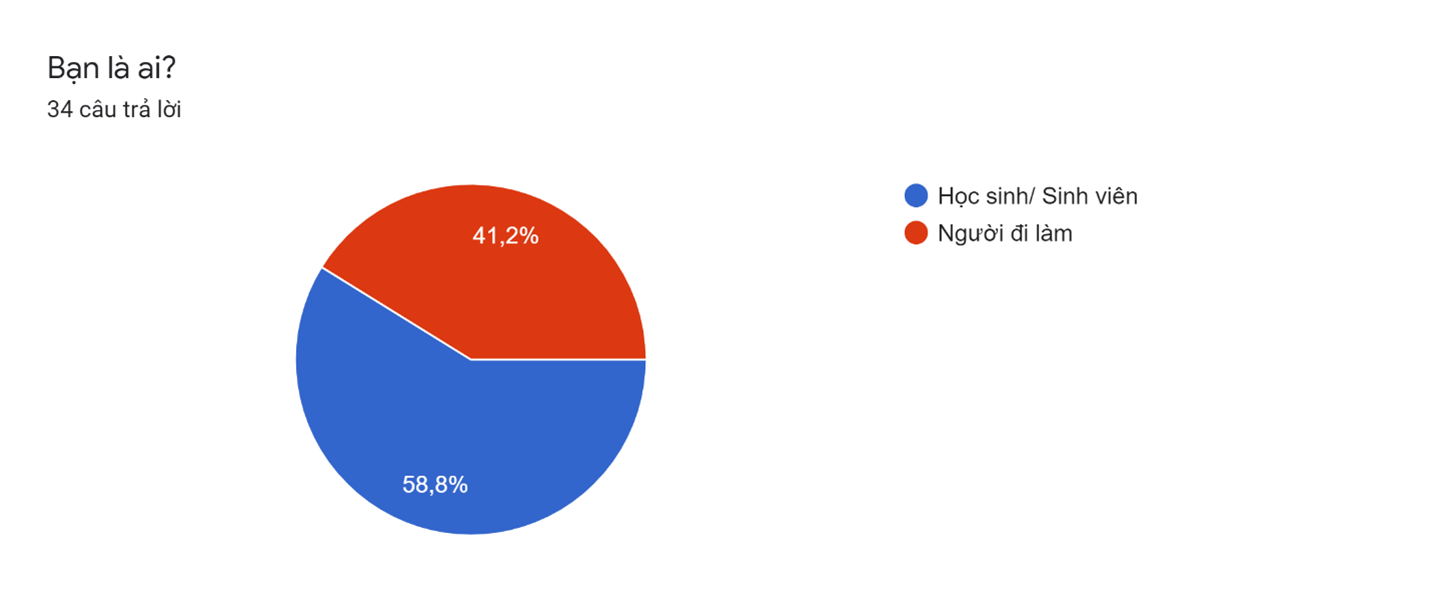
\includegraphics{images/survey1}
\caption{Thống kê đối tượng đang là sinh viên hoặc đã đi làm }
\label{fig:survey1}
\end{figure}
Phần lớn đối tượng tham gia khảo sát là sinh viên chiếm 58.8\% và đối với đối tượng là người đã đi làm thì chiếm 41.2%\\
\pagebreak
\subsection{Bạn hoạt động trong lĩnh vực nào?}
\begin{figure}[htp]
\centering
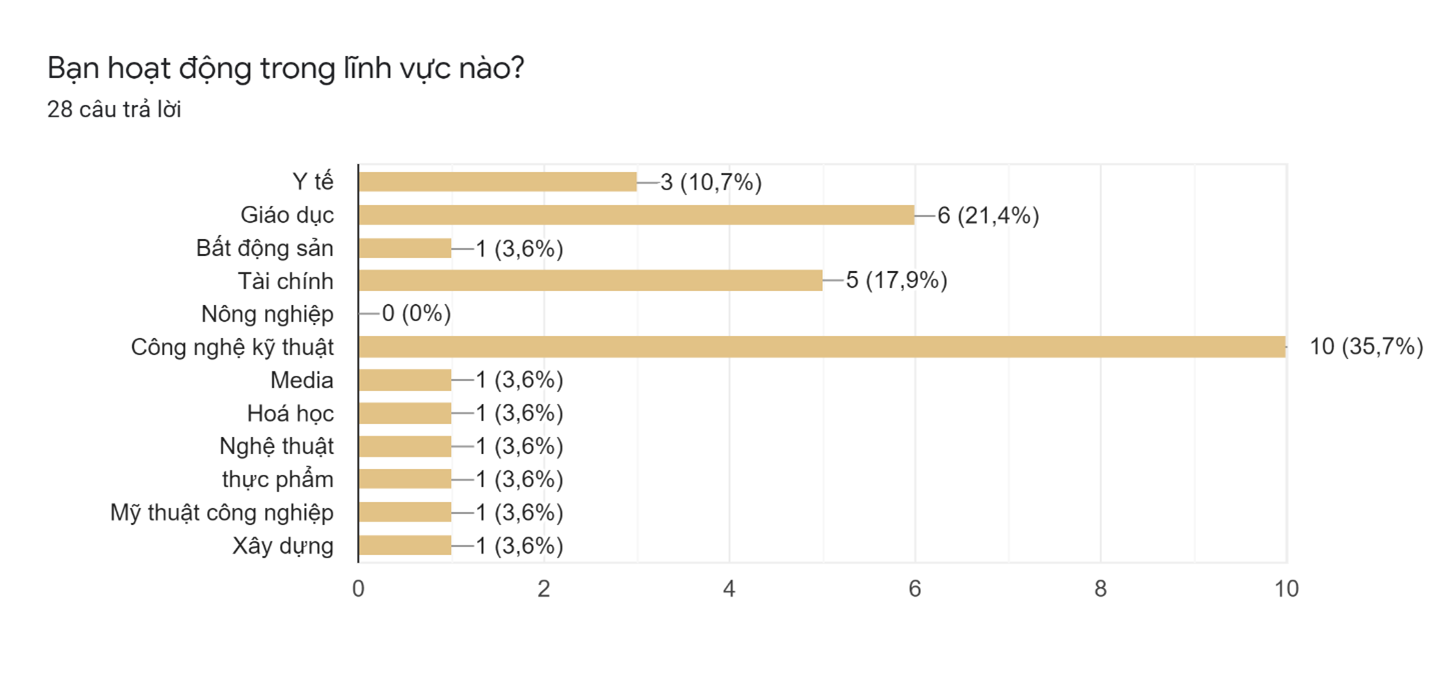
\includegraphics{images/survey2}
\caption{Thống kê đối tượng đang hoạt động trong lĩnh vực nào}
\label{fig:survey2}
\end{figure}

Qua khảo sát cho thấy, người tham gia khảo sát đang hiện hoạt động trong rất nhiều lĩnh vực như Y tế, Giáo dục, Công nghệ kỹ thuật, tài chính chiếm phần trăm khá cao trong tổng số lượng ngành có đưa ra để khảo sát.\\
\pagebreak
\subsection{Bạn đã từng gặp những vấn đề liên quan đến luật pháp?}
\begin{figure}[htp]
	\centering
	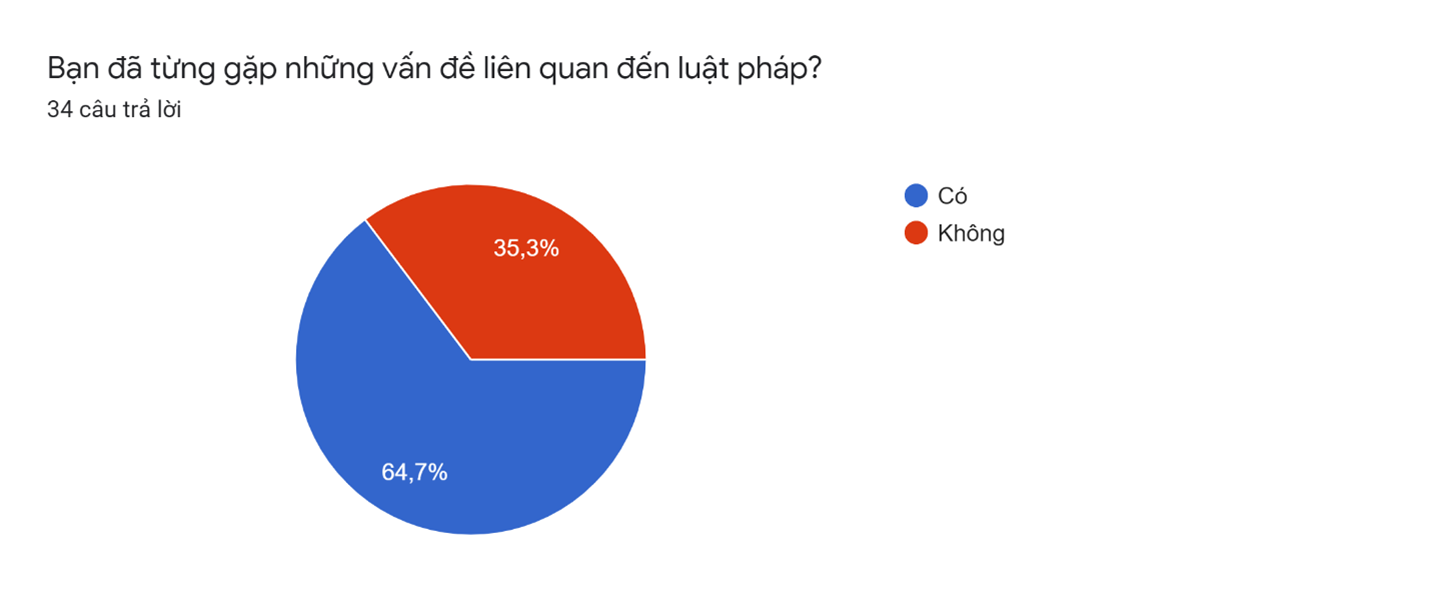
\includegraphics{images/survey3}
	\caption{Thống kê đối tượng có gặp những vấn đề liên quan đến pháp luật không?}
	\label{fig:survey3}
\end{figure}

Dựa vào kết quả khảo sát, có thể thấy đến gần 65\% số người được khảo sát gặp các vấn đề liên quan đến pháp luật, cho dù là học sinh, sinh viên hay người đi làm, học tập, làm việc trong các lĩnh vực khác nhau. Từ đây, có thể thấy nhu cầu tìm hiểu về pháp luật của người thực hiện khảo sát là rất lớn. \\
\pagebreak
\subsection{Bạn sử dụng phương thức nào để tra cứu pháp luật?}

\begin{figure}[htp]
	\centering
	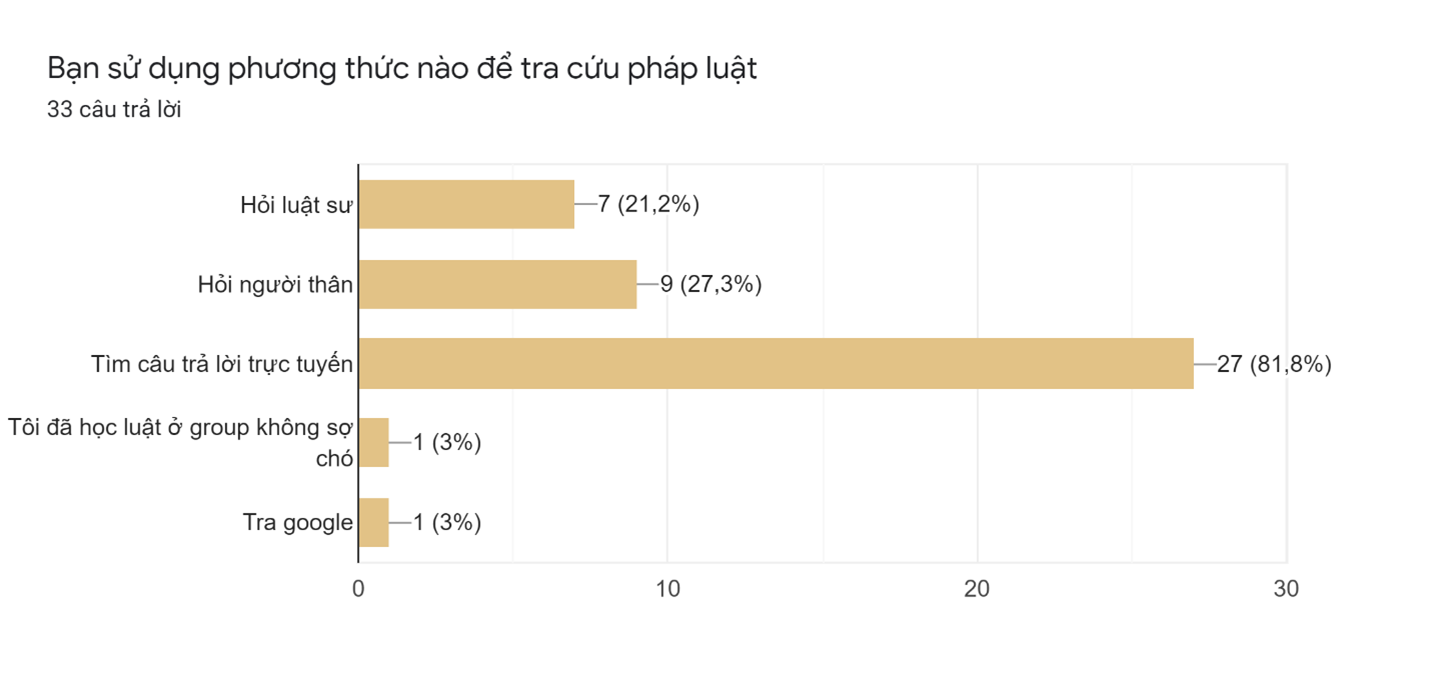
\includegraphics{images/survey4}
	\caption{Thống kê về phương thức nào của người dùng dùng để tra cứu pháp luật}
	\label{fig:survey4}
\end{figure}

Biểu đồ trên cho thấy các phương thức mà người khảo sát sử dụng để tìm hiểu về luật pháp. Đây là câu hỏi người thực hiện khảo sát có thể chọn nhiều phương án, trong đó, có thể thấy rằng người dùng có nhiều phương thức để tra cứu như hỏi luật sư, hỏi người thân,… nhưng đa số vẫn ưa thích tìm câu trả lời trực tuyến thông qua các trang web về pháp luật hoặc tìm trên Google.\\
\pagebreak
\subsection{Bạn thường tra cứu trên trang web pháp luật nào?}

\begin{figure}[htp]
	\centering
	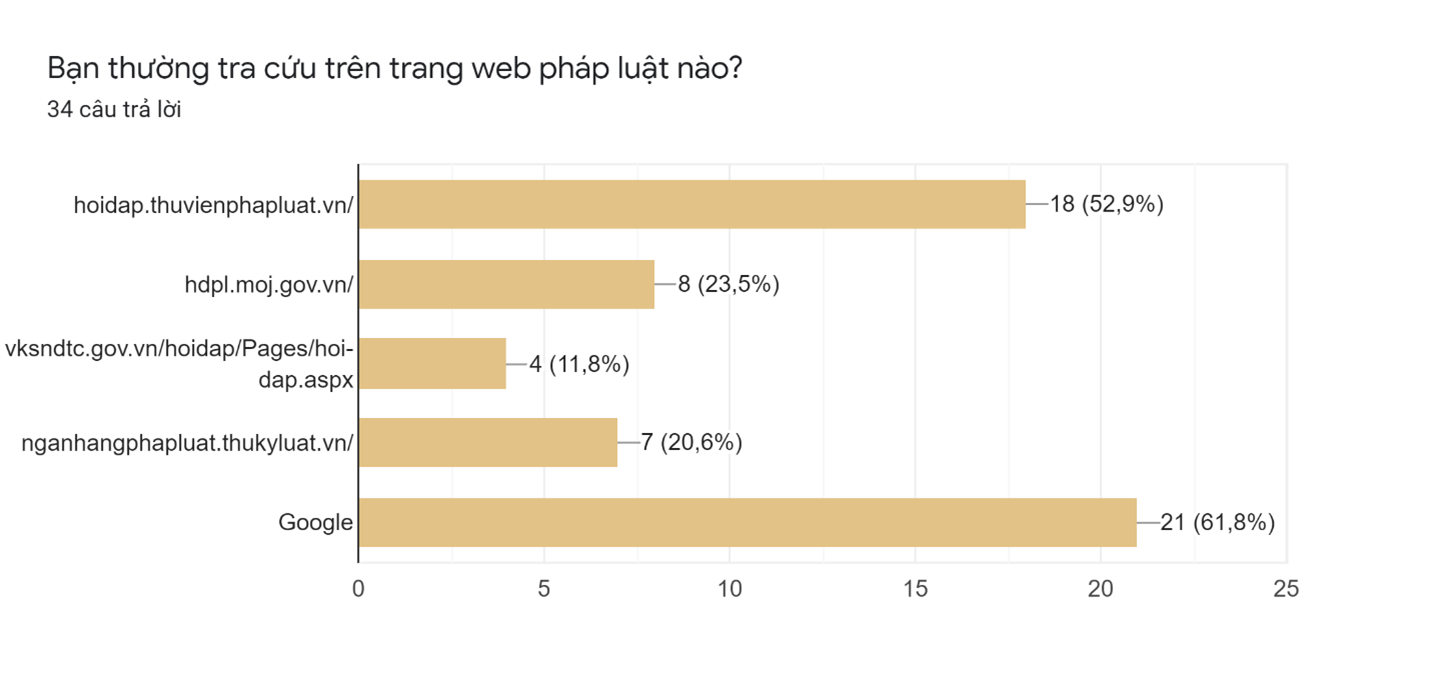
\includegraphics{images/survey5}
	\caption{Thống kê các trang web mà người dùng sử dụng để tra cứu thông tin luật pháp}
	\label{fig:survey5}
\end{figure}

Trên đây là những trang web chứa các thông tin về văn bản, câu hỏi về luật pháp. Người thực hiện khảo sát có thể sử dụng mỗi trang web khác nhau hoặc họ có thể kết hợp nhiều phương thức để tìm hiểu chi tiết, chính xác về vấn đề pháp luật họ gặp phải. Nhưng kết quả phần lớn vẫn là search thông tin của câu hỏi bằng Google.\\
\pagebreak
\subsection{Mức độ hài lòng khi sử dụng các trang web trên?}
\begin{figure}[htp]
	\centering
	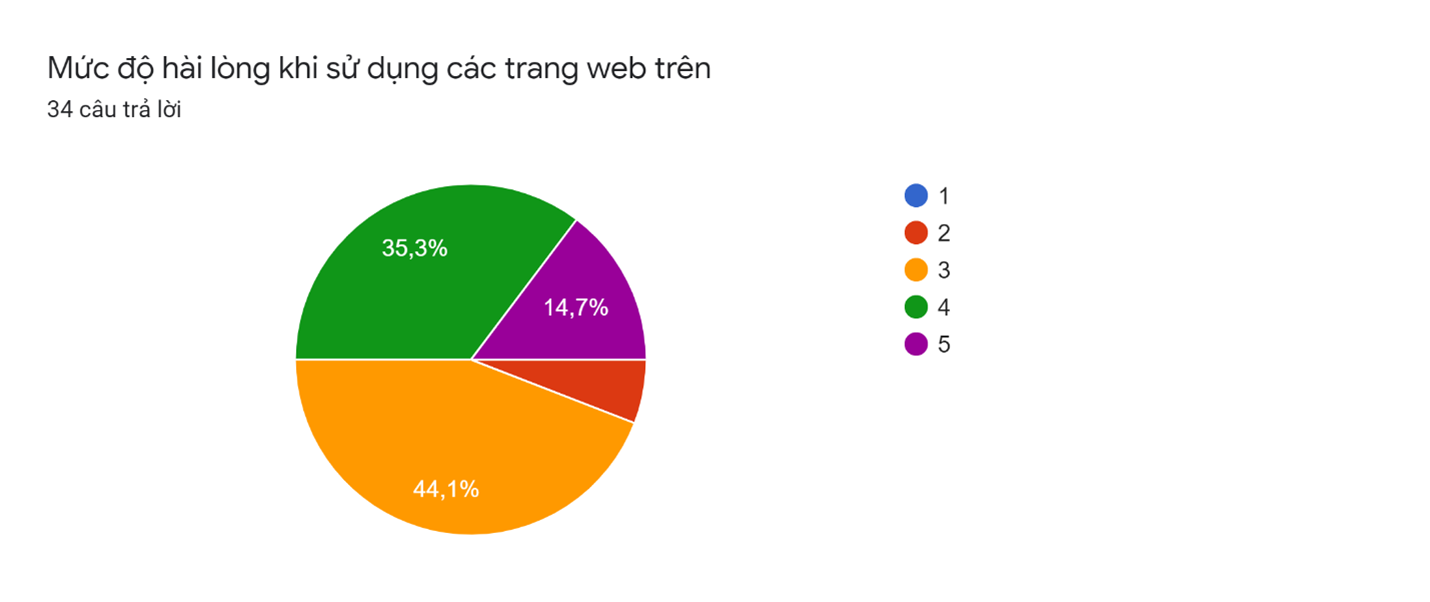
\includegraphics{images/survey6}
	\caption{Thống kê mức độ hài lòng khi sử dụng các trang web trên}
	\label{fig:survey6}
\end{figure}
Sau đó, người thực hiện khảo sát được yêu cầu cho cảm nhận về mức độ hài lòng khi họ sử dụng các trang web trên. Thang điểm từ 1 đến 5, tương ứng với các mức ‘rất tệ’, ‘tệ’, ‘vừa đủ’, ‘tốt’ và ‘rất tốt’. Từ biểu đồ trên, có thể thấy 44,1\% người dùng cảm thấy vừa đủ hài lòng khi sử dụng các trang web. 35,3\% cảm thấy tốt và 14,7\% cảm thấy rất tốt. Bên cạnh đó, họ còn đưa ra các nhận xét tích cực như ‘tiện lợi, nhanh chóng’ hay ‘khá chi tiết, đầy đủ’. Tuy nhiên, có một số nhận xét không hài lòng như khi sử dụng Google để tìm kiếm thông tin, kết quả trả về nhiều, tốn thời gian hoặc có người cho rằng các vấn đề về pháp luật của mỗi người khác nhau nhưng các trang web chỉ đưa ra những câu trả lời chung, khó có thể giải quyết mọi vấn đề.  \\

\subsection{Nhận xét của bạn khi sử dụng các trang web trên}
Mục này người khảo sát trả lời quá ít nên không thể thống kê.

\section{Bài Toán Liên Quan}
Qua quá trình tìm kiếm, tìm hiểu thì nhóm rút ra được để giải quyết được yêu cầu của hệ thống thì sẽ cần giải được các bài toán nhỏ liên quan như sau:
\begin{itemize}
	\item Thu thập giữ liệu về pháp luật từ các trang web chuyên về pháp luật
	\item Mã hoá dữ liệu câu hỏi - Xử lý ngôn ngữ tự nhiên
	\item So sánh tìm ra sự tương đồng giữa các câu
	\item Xây dựng model train trên dữ liệu Pháp luật     
\end{itemize}

\pagebreak


\chapter{Công nghệ sử dụng}
\label{Chapter3}
\textit{Nội dung chương này sẽ đề cập đến các công nghệ sẽ được áp dụng bên trong hệ thống, các phần mềm , thư viện cần để hệ thống hoạt động, cách cài đặt các phần mềm và thư viện cần sử dụng. }

%thư viện requests
\section{Thư viện Requests}
\subsection{Định nghĩa }

Requests là một thư viện trong Python sử dụng để gửi các request HTTP. Request HTTP sẽ trả về một Respond Object với tất cả dữ liệu như nội dung, trạng thái, mã hoá, ... 

Việc sử dụng Requests trong đề tài này là dùng cho việc scraping câu hỏi và câu trả lời pháp luật từ website hỏi đáp pháp luật.

Để tạo một GET request thì chỉ cần import tất cả thư viện của module vào và thực hiện yêu cầu. Ví dụ như là:

\begin{lstlisting}
	import requests
	req = requests.get('https://hoidap.thuvienphapluat.vn/')
\end{lstlisting}

Tất cả các thông tin về yêu cầu của chúng ta bây giờ được lưu trữ trong một đối tượng Response được gọi là req. Vì vậy, để có thể tìm được các thuộc tính của trang web chỉ cần truy cập vào các thuộc tính của trang web có trong đối tượng req.

Việc phân tích, tìm kiếm thông tin trong đối tượng req cũng chính là nội dung chính của việc scraping data từ một website.

Thư viện này sẽ được áp dụng vào trong bài toán thu thập dữ liệu câu hỏi và câu trả lời về Pháp luật ở website cung cấp thông tin về Pháp luật.
%BeautifulSoup
\section{Thư viện BeautifulSoup}

BeautifulSoup\cite{Scraping} là một thư viện của Python nhằm hỗ trợ để bóc tách dữ liệu ra khỏi các file HTML. Nó hoạt động cùng với các \textbf{parser} để điều hướng, tìm kiếm, chỉnh sửa trong parse tree. Các parser khác nhau như là: html.parser, lxml, html5lib.

Parser \textbf{lxml} là một loại parser hỗ trợ trong việc phân tích HTML để phục vụ cho công việc scraping dữ liệu.

Các Object cần quan tâm khi sử dụng BeautifulSoup là:
\begin{itemize}
	\item Tag: tương ứng với một thẻ tag trong tài liệu HTML.
	\item NavigableString: là một chuỗi tương ứng với một bit văn bản có chứa trong một tag.
	\item BeautifulSoup: là một đối tượng đại diện cho toàn bộ tài liệu.
	\item Comment: là một dạng đặc biệt của NavigableString, cho phép truy cập vào các comment của một file HTML.
\end{itemize}

Thư viện này sẽ được áp dụng vào trong bài toán thu thập dữ liệu câu hỏi và câu trả lời về Pháp luật ở website cung cấp thông tin về Pháp luật.
%Python Vietnamese Toolkit
\section{Phân tách từ bằng Python Vietnamese Toolkit}
\subsection{Định nghĩa PyVi}
Python Vietnamese Toolkit(PyVi)\cite{pyvi} là một công cụ xử lý ngôn ngữ tự nhiên dùng cho tiếng Việt với các hàm xử lý như:

\begin{itemize}
	\item Tokenization: tách từ, cụm từ trong văn bản
	\item POS tagging: gán nhãn từ loại, các loại từ bao gồm: A – Adjective: tính từ, C – Coordinating conjunction: liên từ, E – Preposition: giới từ, I – Interjection: thán từ,L – Determiner: từ hạn định, M – Numeral: số, N - Common noun: danh từ chung, Nc - Noun Classifier: phân loại danh từ, Ny - Noun abbreviation: các danh từ viết tắt, Np - Proper noun: danh từ riêng, Nu - Unit noun: danh từ đơn vị, P – Pronoun: đại từ, R – Adverb: trạng từ, S - Subordinating conjunction:  liên từ phụ thuộc, T - Auxiliary, modal words: động từ khiếm khuyết, V – Verb: động từ, X – Unknown: các từ không xác định được, F - Filtered out (punctuation): các từ được lọc ra bởi dấu chấm câu
	\item Accents removal: bỏ dấu từ
	\item Accents adding: thêm dấu từ
	
\end{itemize}

\begin{figure*}[htp]
    \centering
    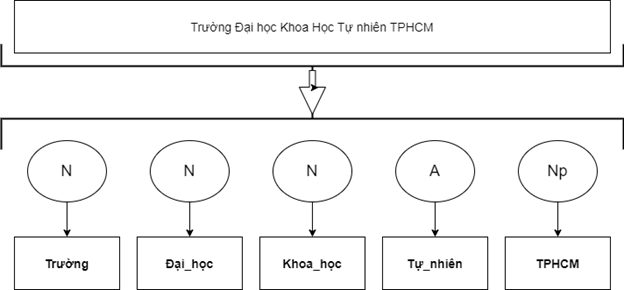
\includegraphics[scale=0.7]{images/pyvi_segment}
    \caption{Minh hoạ tách từ bằng PyVi.}
    \label{fig:ex_pyvi_1}
\end{figure*}
\pagebreak
\subsection{Tính năng chính của PyVi}
Sau đây là một đoạn code mẫu mô tả cách sử dụng và kết quả trả về của PyVi:
%biện pháp thay thế cho code bị lỗi encode utf-8
\begin{figure*}[htp]
	\centering
	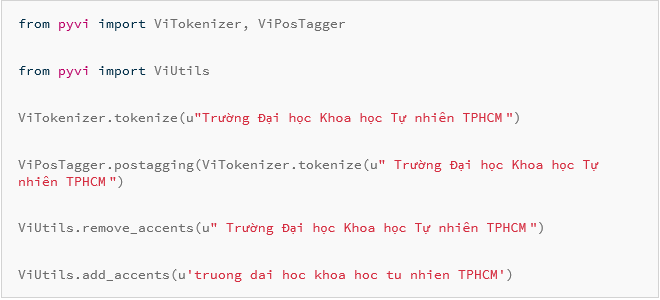
\includegraphics[scale=0.85]{images/pyvi_demo_code}
\end{figure*}

\hfill 

Khi chạy đoạn code trên, ta sẽ thu được các kết quả như:

Tokenize (tách từ):

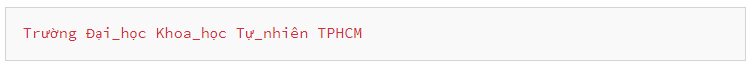
\includegraphics[scale=0.7]{images/segment1}

POS\_tagging (gán nhãn từ loại): khi thực hiện POS tagging thì hàm sẽ thực hiện tách từ (Tokenize) trước khi trả về kết quả. Kết quả trả về gồm mảng 2 chiều với thứ tự gán nhãn tương ứng với nhau:

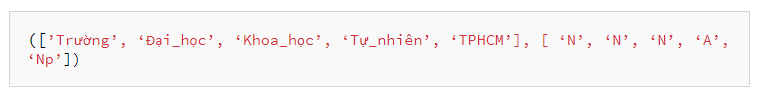
\includegraphics[scale=0.7]{images/segment2}

Accents removal (bỏ dấu):

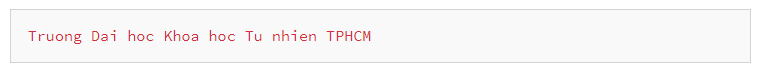
\includegraphics[scale=0.7]{images/segment3}

Accents adding(Thêm dấu):

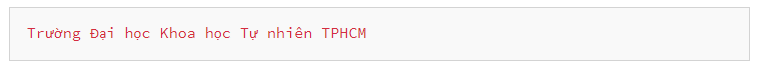
\includegraphics[scale=0.7]{images/segment4.png}

Thư viện này sẽ được áp dụng vào trong bài toán xử lý ngôn ngữ tự nhiên(tách từ ghép trong tiếng Việt).
%transformer
\section{Mô hình Transformer}
\subsection{Định nghĩa mô hình Transformer}
Trước khi Transformers xuất hiện, đa số các tác vụ xử lý ngôn ngữ tự nhiên sử dụng kiến trúc của Recurrent Neural Networks(RNNs) – Mạng nơ-ron hồi quy. Điểm yếu của RNNs là khó nắm bắt được sự phụ thuộc xa giữa các từ trong câu và tốc độ huấn luyện mô hình chậm do phải xử lý tuần tự. Transformers có thể giải quyết các vấn đề này.

Transformers ra đời nhằm giải quyết vấn đề chuyển đổi chuỗi dữ liệu hoặc dịch máy, chẳng hạn như các bài toán như nhận dạng giọng nói, chuyển văn bản thành giọng nói,…
	
Kiến trúc của Transformers bao gồm hai phần là Encoder và Decoder, Encoder dùng để học, chuyển hoá vector biểu diễn của câu văn bản và Decoder sẽ thực hiện biểu diễn vector dó dưới ngôn ngữ của người dùng.

\pagebreak
\subsection{Ưu điểm của Transformers}
Ưu điểm của Transformers là mô hình này có khả năng xử lý song song cho các từ trong câu văn bản, gia tăng hiệu suất và giảm thời gian huấn luyện.

\begin{figure*}[htp]
    \centering
    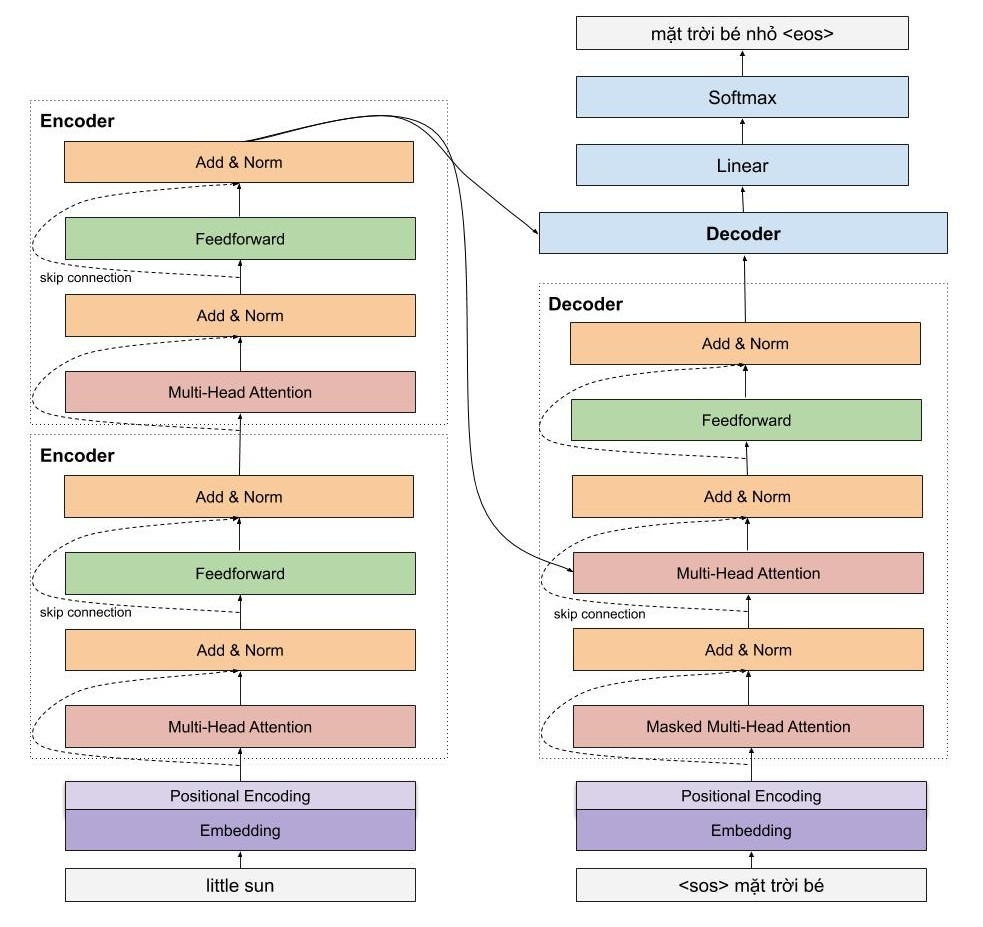
\includegraphics[width=13 cm, height=15 cm]{images/transformer_schema}
    \caption{Mô hình tổng quát của cấu trúc của Transformer.}
    \label{fig:transformer_schema}
\end{figure*}


Ý tưởng của mô hình Transformers là áp dụng cơ chế Attention. Chính thành phần Multi-Head Attention trong các lớp Encoder cho phép mô hình mã hoá một từ có thể sử dụng thông tin của những từ liên quan đến nó.

Mô hình này sẽ được áp dụng vào trong bài toán mã hoá dữ liệu câu hỏi Pháp luật.
\pagebreak


%BERT MODEL

\section{Mô hình BERT}
\subsection{Định nghĩa mô hình BERT}
BERT là viết tắt của “Bidirectional Encoder Representations from Transformers”, là một mô hình học sẵn, học biểu diễn vector đại diện cho câu theo ngữ cảnh 2 chiều.

Một trong những khó khăn khi xử lý ngôn ngữ tự nhiên đó là việc thiếu hụt dữ liệu gán nhãn. Hầu hết các dữ liệu đều được gán nhãn thủ công bởi con người, vì vậy, số lượng mẫu dữ liệu chất lượng không nhiều. Do đó, để giải quyết vấn đề này, các mô hình xử lý ngôn ngữ tự nhiên sử dụng cơ chế tiền xử lý dữ liệu, cơ chế này tạo ra một mô hình chung được huấn luyện từ số lượng lớn dữ liệu không gán nhãn, chẳng hạn như các mô hình Word2Vec, Glove,… Tuy nhiên, các mô hình này thường không biểu diễn chính xác ngữ nghĩa của từ trong ngữ cảnh câu văn bản, dẫn đến khó khăn trong việc xác định nghĩa của một từ đang được đề cập trong ngữ cảnh nào.

BERT có khả năng tạo ra mô hình ngôn ngữ cho phép các hệ thống tìm kiếm hiểu rõ hơn về ngữ nghĩa của từ trong câu dựa vào xem xét mối liên hệ giữa các từ trước và sau của từ đó.  

BERT được xây dựng dựa trên Transformers với hai biến thể:
\begin{itemize}
    \item BERT$_{BASE}$ gồm 12 lớp Encoder, kích thước của các lớp ẩn là 768 với 110 triệu tham số. 
    \item BERT$_{LARGE}$ gồm 24 lớp Encoder, kích thước của các lớp ẩn là 1024 với 340 triệu tham số
\end{itemize}
\begin{figure*}[htp]
    \centering
    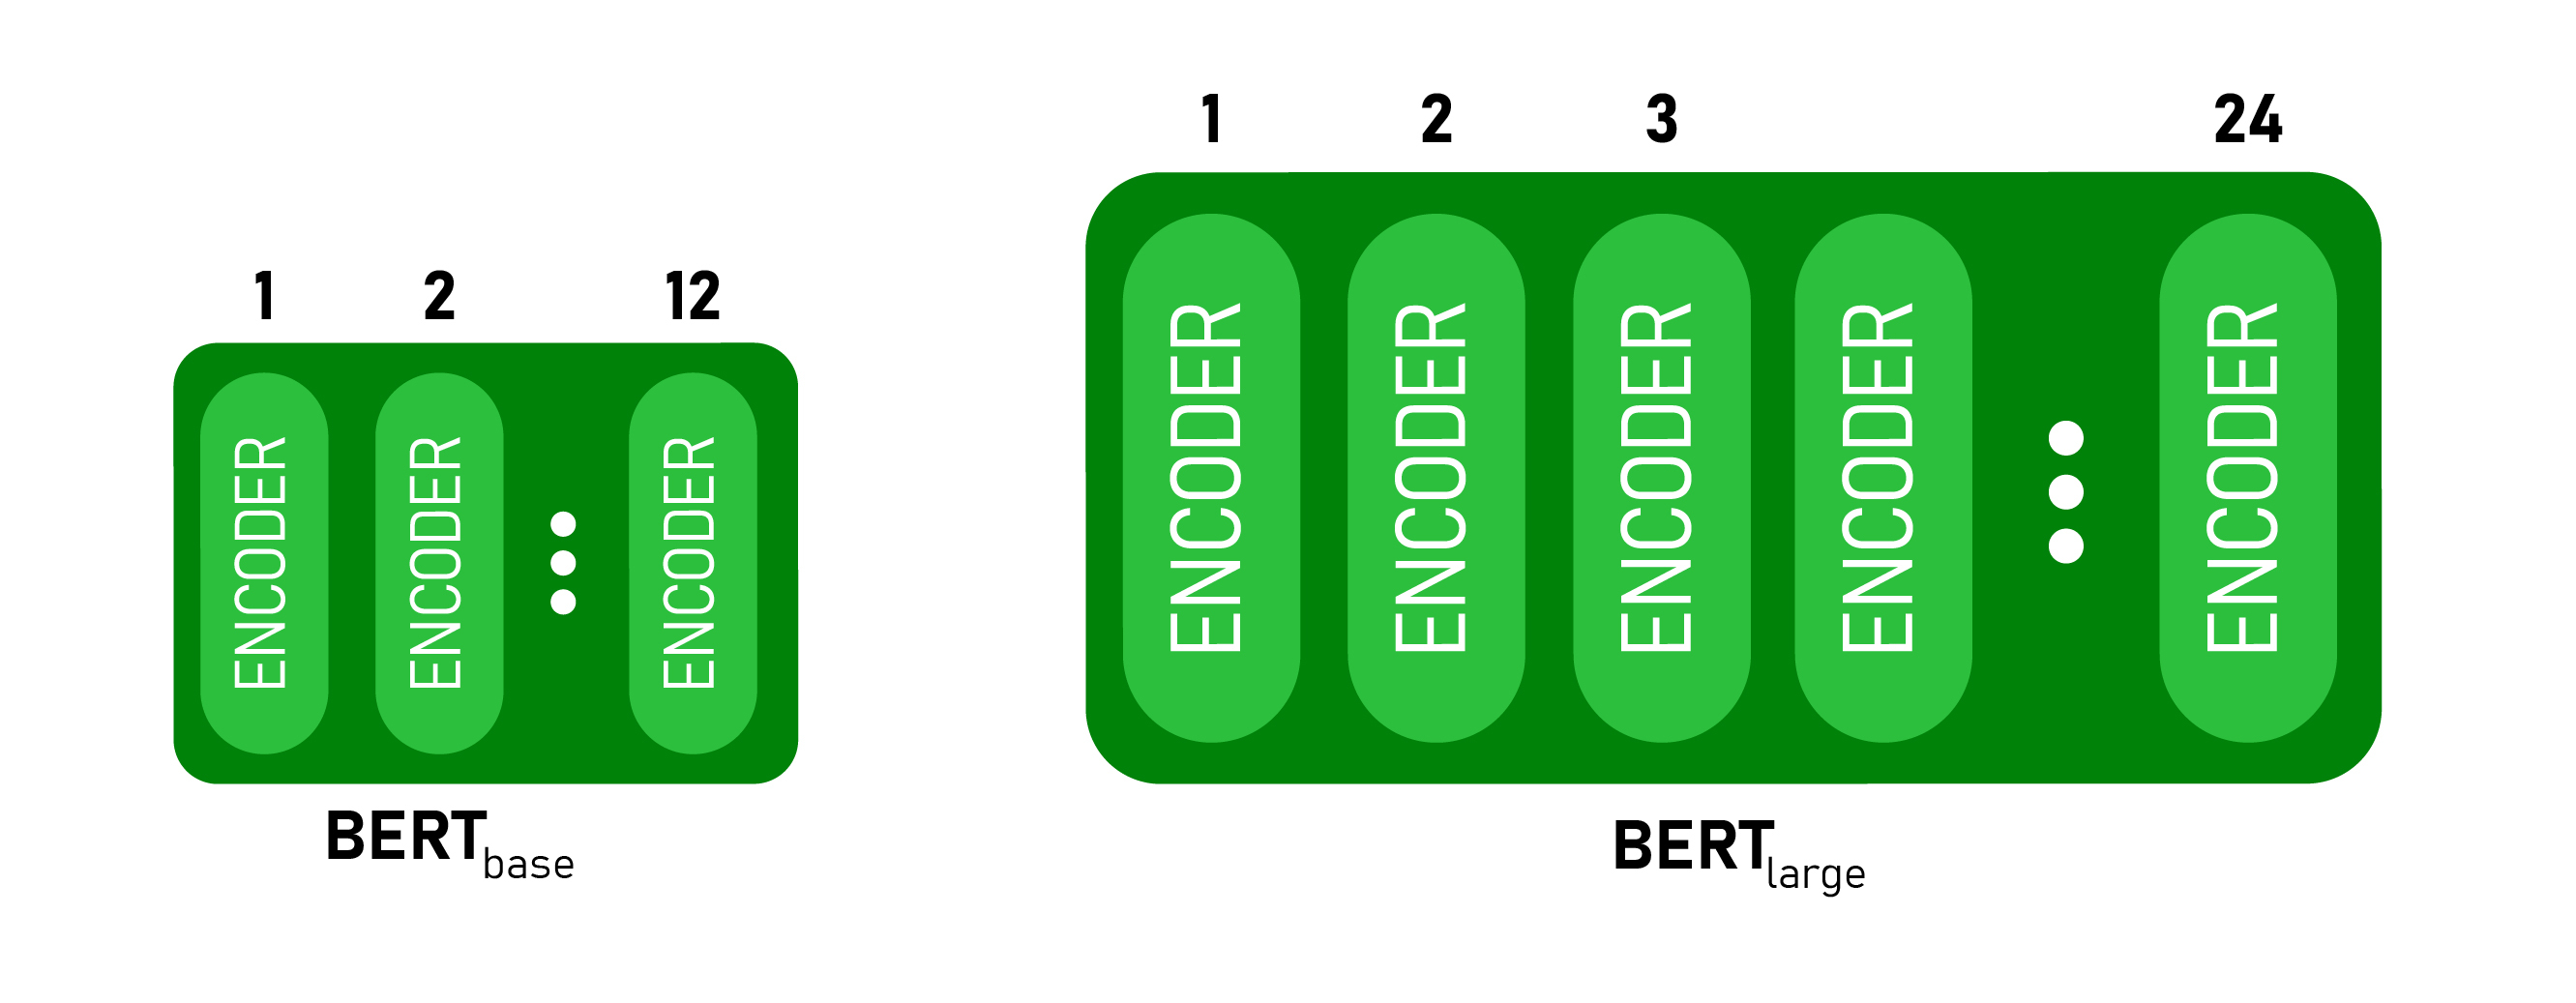
\includegraphics[scale=0.1]{images/bert-base-and-large.jpg}
    \caption{Kích thước của 2 dạng BERT.}
    \label{fig:BERT_SIZE}
\end{figure*}

Trong khi đó kiến trúc của Transformers chỉ có 6 lớp Encoder, cho thấy khả năng xử lý của BERT mang lại hiệu suất cao hơn.
\begin{figure*}[htp]
    \centering
    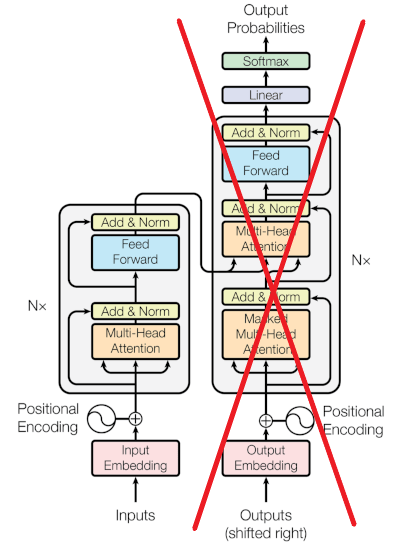
\includegraphics[width=12.5 cm, height=17 cm]{images/encode_bert.png}
    \caption{Encode BERT.}
    \label{fig:encode_bert}
\end{figure*}


Kiến trúc của BERT khác với Transformers ở chỗ nó chỉ dùng thành phần Encoder của Transformers vì mục tiêu sử dụng BERT là để tạo ra được một mô hình thực hiện các tác vụ NLP khác nhau. Việc sử dụng Encoder cho phép BERT mã hóa thông tin ngữ nghĩa, cú pháp của câu trong quá trình nhúng. 

BERT không sử dụng thành phần Decoder của Transformers nên kết quả đầu ra của nó là một embedding – một không gian vector dùng để biểu diễn dữ liệu có thông tin về mối liên hệ, sự tương đồng về mặt ngữ nghĩa, ngữ cảnh của dữ liệu, trong đó bao gồm nhiều chiều và các từ có sự tương đồng sẽ có vị trí gần nhau. Vì kết quả đầu ra của BERT là word embedding nên người sử dụng có thể làm các tác vụ khác nhau. Người dùng có thể sử dụng các kỹ thuật để tính sự tương đồng, chẳng hạn như Cosine Similarity để so sánh giữa các vector đại diện và trả về điểm số tương đồng.

Mô hình này sẽ được áp dụng vào trong bài toán mã hoá dữ liệu câu hỏi Pháp luật.
%Sentence-transformer
\section{Sentence-transformer}
Sentence Transformers\cite{sentencetransformer} là 1 framework dùng để Embedd (nhúng) những câu văn, đoạn văn, hình ảnh để tạo ra các Embeddings có ý nghĩa về mặt ngữ nghĩa, được sử dụng để áp dụng cho các bài toán, ứng dụng Semantic Search (tìm kiếm ngữ nghĩa) hoặc là Multi-lingual Zero-shot Classification (phân loại Zero-shot đa ngôn ngữ).

Sentence Transformers là phương pháp để tính toán, tạo ra các vector biểu diễn cho các câu văn, đoạn văn bản hay là một hình ảnh. Các mô hình như BERT, RoBERTa, XLM-RoBERTa,... đều dựa trên framework Sentence Transformers này. Các đoạn văn bản sau khi được Vector hóa có thể tìm được sự tương đồng về mặt ngữ nghĩa với nhau bằng cách dùng phương pháp tính Cosine Similarity.

Như vậy với Sentence Transformers, ta có thể:

Dùng các độ đo khoảng cách hoặc góc để tính độ tương đồng về ngữ nghĩa của các câu, áp dụng để phân nhóm câu theo ngữ nghĩa (Semantic Clustering), dùng trong Hệ thống truy vấn thông tin theo ngữ nghĩa (Semantic Information Retrieval), tính toán câu tương tự (Computing Sentence Similarity), ...

Sử dụng như Pre-trained Model trong các Transfer Learning, đã có hơn 100 ngôn ngữ được huấn luyện sẵn nên rất dễ cho việc sử dụng.

\pagebreak
Ví dụ về sử dụng mô hình Sentence Transformer để nhúng (Embedd) các câu văn:
\begin{lstlisting}[language=python]
from sentence_transformers import SentenceTransformer
sentences = ["There was coal in his stocking and he was thrilled"]
model = SentenceTransformer('paraphrase-MiniLM-L6-v2')
embeddings = model.encode(sentences)
print("Sentence: ", sentences)
print("Embedding: ", embeddings)
\end{lstlisting}

Và đây là kết quả:
\begin{lstlisting}
Sentence:  ['There was coal in his stocking and he was thrilled']
	Embedding: [[-3.29191387e-01  1.03968787e+00 -2.23834172e-01  7.96381384e-02
	-7.98925042e-01 -1.18792735e-01  7.98527181e-01  3.68809402e-01
	-1.13197708e+00  9.99245495e-02 -5.30997992e-01 -2.71604806e-01
	-1.89905569e-01 -7.41842622e-03 -3.44552487e-01  5.15601277e-01...]]	
\end{lstlisting}

%Phở bert
\section{Mô hình PhoBERT}

PhoBERT\cite{PhoBERT},\cite{PhoBERT_VNMESE}  là một pre-trained model dựa trên BERT, được xây dựng để huấn luyện riêng cho ngôn ngữ tiếng Việt, dựa trên kiến trúc RoBERTa – model tương tự BERT nhưng có phần tối ưu quá trình tiền huấn luyện cho hiệu suất cao do kiến trúc này đã bỏ đi tác vụ Next Sentence Prediction. 

PhoBERT cũng có hai kích thước là PhoBERT$_{BASE}$ với 12 transformers block và PhoBERT$_{LARGE}$ với 24 transformers block. PhoBERT được huấn luyện từ 20GB dữ liệu về Tiếng Việt bao gồm 1GB Vietnamese Wikipedia corpus và 19GB Vietnamese news corpus. 

PhoBERT sử dụng RDR Segmenter của VnCoreNLP để tách từ cho dữ liệu đầu vào trước khi qua BPE encoder. PhoBERT tượng tự BERT, chỉ khác là dùng cho việc xử lý ngôn ngữ tiếng Việt nên kiến trúc của PhoBERT cũng thừa hưởng thành phần Encoder của mô hình Transformers, không bao gồm Decoder.

Mô hình này sẽ được áp dụng vào trong bài toán mã hoá dữ liệu câu hỏi Pháp luật.
%SimCSE
\section{Pre-trained model SimCSE}

SimCSE\cite{gao2021simcse} là một pre-trained model sử dụng PhoBERT, dùng để mã hóa câu, đoạn văn bản dữ liệu đầu vào. SimCSE cho hiệu suất huấn luyện cao hơn, làm việc đồng thời với cả hai loại dữ liệu đã được gắn nhãn hoặc không.

Việc áp dụng mô hình SimCSE là cần thiết vì đây là mô hình sử dụng các phương pháp kỹ thuật hiện đại nhất trong tác vụ xử lý dữ liệu đầu vào. Thêm vào đó, với tác vụ đánh giá sự tương đồng ngữ cảnh giữa các câu văn bản, SimCSE mang lại kết quả khá cao so với BERT.

Mô hình này sẽ được áp dụng vào trong bài toán mã hoá dữ liệu câu hỏi Pháp luật.
%Elasticsearch
\section{Elasticsearch}
Elasticsearch là một công cụ tìm kiếm dựa trên nền tảng Apache Lucene. Nó cung cấp một bộ máy tìm kiếm dạng phân tán, có đầy đủ công cụ với một giao diện web HTTP có hỗ trợ dữ liệu JSON.

Elasticsearch chạy trên server riêng và đồng thời giao tiếp thông qua RESTful do vậy nên nó không phụ thuộc vào client viết bằng gì hay hệ thống hiện tại của bạn viết bằng gì. Nên việc tích hợp nó vào hệ thống bạn là dễ dàng, bạn chỉ cần gửi request http lên là nó trả về kết quả.

Các khái niệm cần phải biết khi sử dụng Elasticsearch\cite{ES} là:
\begin{itemize}
	\item Document: là một Object JSON, có thể xem là đơn vị lưu trữ nhỏ nhất của Elasticsearch
	\item Index: được xem như là một "database" khi quy chiếu sang với cơ sở dữ liệu quan hệ.
	\item Shard: là khối các Elasticsearch với mục đích mở rộng, nâng cấp.
	\item Node: Là trung tâm hoạt động của Elasticsearch. Là nơi lưu trữ dữ liễu ,tham gia thực hiện đánh index của cluster cũng như thực hiện các thao tác tìm kiếm.
	\item Cluster: là tập hợp các nodes hoạt động cùng với nha. Mỗi Cluster có một Node chính được chọn một cách tự động và có thể thay thay thế nếu có sự cố xảy ra.
\end{itemize}

Chức năng chính của Cluster đó chính là quyết định xem shards nào được phân bổ cho node nào và khi nào thì di chuyển các Cluster để cân bằng lại Cluster.

\subsection{Ưu điểm của Elasticsearch}
Tìm kiếm dữ liệu rất nhanh chóng, mạnh mẽ dựa trên Apache Lucene ( near-realtime searching)

Có khả năng phân tích dữ liệu (Analysis data)

Khả năng mở rộng theo chiều ngang

Hỗ trợ tìm kiếm mờ (fuzzy), tức là từ khóa tìm kiếm có thể bị sai lỗi chính tả hay không đúng cú pháp thì vẫn có khả năng Elasticsearch trả về kết quả tốt.

Hỗ trợ Structured Query DSL (Domain-Specific Language ), cung cấp việc đặc tả những câu truy vấn phức tạp một cách cụ thể và rõ ràng bằng JSON.

Hỗ trợ nhiều Elasticsearch client như Java, PhP, Javascript, Ruby, .NET, Python

\subsection{Nhược điểm của Elasticsearch}

Elasticsearch được thiết kế cho mục đích search, do vậy với những nhiệm vụ khác ngoài search như CRUD thì elastic kém thế hơn so với những database khác như Mongodb, Mysql …. Do vậy người ta ít khi dùng Elasticsearch làm database chính, mà thường kết hợp nó với 1 database khác.

Trong Elasticsearch không có khái niệm database transaction , tức là nó sẽ không đảm bảo được toàn vẹn dữ liệu trong các hoạt độngInsert, Update, Delete.Tức khi chúng ta thực hiện thay đổi nhiều bản ghi nếu xảy ra lỗi thì sẽ làm cho logic của mình bị sai hay dẫn tới mất mát dữ liệu. Đây cũng là 1 phần khiến Elasticsearch không nên là database chính.

Không thích hợp với những hệ thống thường xuyên cập nhật dữ liệu. Sẽ rất tốn kém cho việc đánh index dữ liệu.	

%Flask
\section{Web Framework: Flask Framework}
\begin{enumerate}
    \item Flask Framework:
    \begin{figure*}[htp]
        \centering
        
\includegraphics{images/Flask_Logo}
        \caption{Flask logo.}
        \label{fig:flask_logo}
    \end{figure*}
    

Flask là một Web Frameworks, được xây dựng bằng ngôn ngữ lập trình Python.
         
Flask dựa trên bộ công cụ \textbf{Werkzeg WSGI} và template engine \textbf{Jinja2}:

\textbf{WSGI} (Web Server Gateway Interface): WSGI là Giao diện Cổng Máy chủ Web, WSGI mô tả cách máy chủ web giao tiếp với các ứng dụng web và cách các ứng dụng web có thể được kết nối với nhau khi xử lý một yêu cầu.

\textbf{Werkzeug}: Werkzeug là một bộ công cụ WSGI thực hiện các yêu cầu, đối tượng phản hồi và các chức năng tiện ích, cho phép xây dựng một Web Framework trên đó. Flask framework sử dụng Werkzeg làm một trong những cơ sở của nó.

\textbf{jinja2}: jinja2 là một template engine phổ biến cho Python, được sử dụng để hiển thị dữ liệu cho các trang web. Jinja2 cho phép chuyển các biến Python vào các HTML template – thuận tiện cho việc đổ dữ liệu từ Back End đến Front End.

Flask cung cấp các thư viện, công cụ, cơ chế để xây dựng các Website từ nhỏ đến lớn, từ đơn giản tới phức tạp như: các API nhỏ, trang blog, trang web thương mại điện tử,…
        
Flask thuộc loại Micro-framework: có ưu điểm là rất nhẹ và nhỏ, không phụ thuộc vào thư viện bên ngoài nên rất ít lỗi, do đó dễ dàng đề phòng, phát hiện và xử lý các lỗi bảo mật
    
    
\item Ví dụ web API đơn giản xây dựng bằng Flask\cite{FlaskAPIWeb}:
Sau đây là một đoạn code để tạo một Route của một website

%code        
\begin{lstlisting}[language=Python]
from flask import Flask 
app = Flask(__name__) 
@app.route('/hello') 
def hello_world(): 
	return 'Hello, World!' 
if __name__ == '__main__': 
	app.run(host='0.0.0.0', port=5001)
\end{lstlisting}
    
Để khởi tạo instance của class, dòng code dưới sẽ tạo một web server điều hướng các request từ client đến ứng dụng của chúng ta, nó cũng là chính là một ứng dụng WSGI(Web Server Gateway Interface):
%code
\begin{lstlisting}[language=Python]
    app = Flask(__name__):
\end{lstlisting}

Route decorator cho FLask biết được url nào ứng với hàm nào, Web Server dựa vào đường dẫn và route decorator để chuyển yêu cầu tới hàm xử lý tương ứng $ hello\_world()$, hàm này đóng vai trò làm ứng dụng web (web application).
        
\begin{lstlisting}[language=Python]
    @app.route('/hello') 
\end{lstlisting}

Flask app được chạy với lệnh app.run(). Các tham số trong hàm run:

\begin{lstlisting}
    if __name__ == '__main__': 
	    app.run(host='0.0.0.0', port=5001)
\end{lstlisting}

	\textbf{Host= $'0.0.0.0'$}: Địa chỉ IP để ứng dụng Flask lắng nghe các kết nối, mặc định giá trị của tham số này là $'127.0.0.1'$ và ứng dụng flask chỉ chấp nhận các kết nối từ máy local. chuyển giá trị này thành $'0.0.0.0'$ để ứng dụng chấp nhận các kết nối từ bên ngoài.
	
	\textbf{port=5001}: Giá trị của port là một số nguyên, giá trị mặc định bằng 5001. Là cổng được mở trên máy mà ứng dụng Flask chạy, cần chọn cổng mà chưa được mở trên máy để tránh gặp lỗi khi chạy.
	


\end{enumerate}

%table 3
\section{Hướng dẫn cài đặt các phần mềm cần thiết}
\subsubsection{ElasticSearch}
Truy cập: \url{https://www.elastic.co/downloads/elasticsearch} và tải bản phù hợp với hệ điều hành tại mục Downloads:

\begin{figure*}[htp]
	\centering
	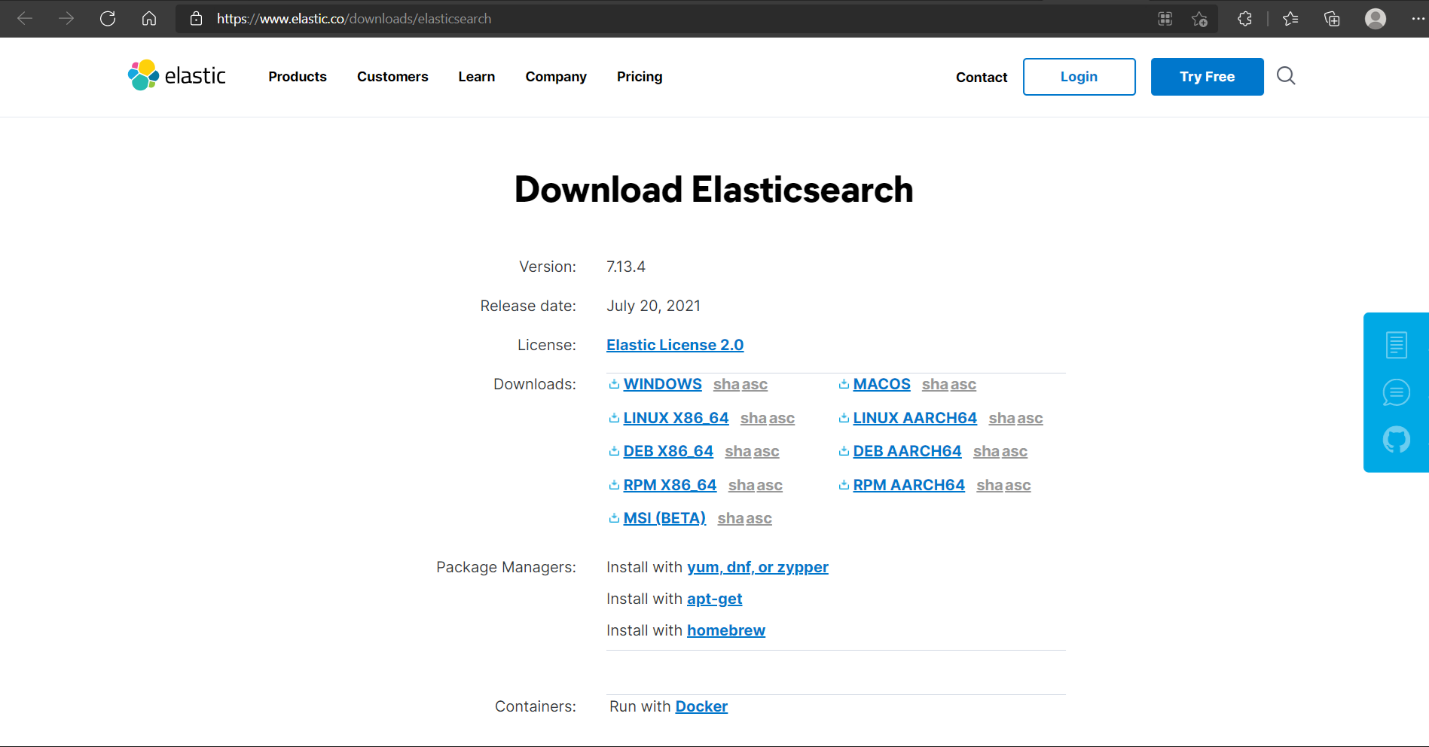
\includegraphics[scale=0.7]{images/elasticsearch1}
	\caption {Giao diện tải về Elastic search.}
	\label{fig:elasticsearch1}
\end{figure*}

Giải nén file .zip vừa tải về thành công ta được thư mục tương ứng

Vào thư mục giải nén:  bin và chạy file elasticsearch.bat

Mở trình duyệt truy cập: \url{http://localhost:9200/} để kiểm tra ElasticSearch đã chạy hay chưa, nếu thành công:

\begin{figure*}[htp]
	\centering
	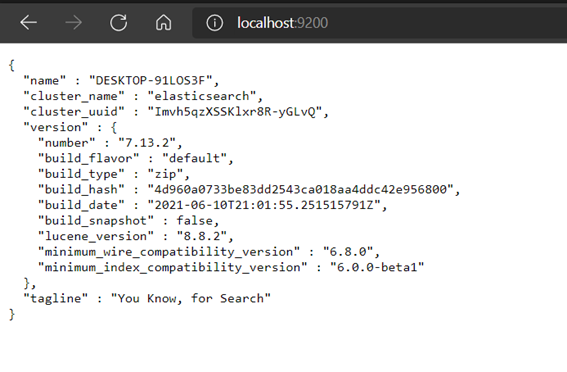
\includegraphics[scale=0.8]{images/elasticsearch2}
	\caption{Trả về kết quả là Elastic search được cài đặt thành công và đang hoạt động.}
\end{figure*}

\subsubsection{Cài đặt các thư viện cần thiết}
\textbf{BeautifulSoup}
\begin{lstlisting}
	pip install beautifulsoup4
\end{lstlisting}

\textbf{Flask 2.0.1}
\begin{lstlisting}
	pip install Flask
\end{lstlisting}

\textbf{utils 1.0.1}
\begin{lstlisting}
	pip install utils
\end{lstlisting}

\textbf{pandas 1.3.1}
\begin{lstlisting}
	pip install pandas
\end{lstlisting}

\textbf{elasticsearch}
\begin{lstlisting}
	pip install elasticsearch
\end{lstlisting}

\textbf{sentence-transformers 2.0.0}
\begin{lstlisting}
	pip install sentence-transformers
\end{lstlisting}

\textbf{pyvi 0.1.1}
\begin{lstlisting}
	pip install pyvi
\end{lstlisting}

\textbf{sklearn}
\begin{lstlisting}
	pip install sklearn
\end{lstlisting}

\textbf{numpy}
\begin{lstlisting}
	pip install numpy
\end{lstlisting}

\textbf{typing}
\begin{lstlisting}
	pip install typing
\end{lstlisting}

\textbf{requests}
\begin{lstlisting}
	pip install requests
\end{lstlisting}


Khi cài thành công các thư viện trên, khi import các thư viện vào trong hệ thống và chạy hệ thống sẽ không có báo lỗi xảy ra khi chạy.\newline

Trong 3 chương tiếp theo, nhóm sẽ tiếp tục trình bày rõ từng bước mà hệ thống sẽ thực hiện, hoạt động, kết quả của từng bước có trong hệ thống.

\chapter{Kiến trúc phần Back-end}
\label{Chapter3}
Ở chương này, nhóm sẽ tập trung giải thích về cách thức hoạt động của phần Back-end của hệ thống. Gồm các giai đoạn như sau:
\begin{itemize}
	\item Xử lý dữ liệu thu thập: Mã hoá dữ liệu đã thu thập ở chương 3, lưu trữ dữ liệu vào trong cơ sở dữ liệu.
	\item Xử lý dữ liệu câu hỏi mà người dùng nhập vào trong hệ thống, cách mà hệ thống xử lý câu hỏi của người dùng và đưa ra kết quả cho người dùng.
	

\end{itemize}
\section{Xử lý dữ liệu thu thập}
Trong mục này, xử lý dữ liệu thu thập là tiến hành việc công việc phân loại từ câu hỏi, mã hoá câu hỏi từ dữ liệu bộ câu hỏi và câu trả lời đã thu thập được ở chương 3 và việc lưu trữ dữ liệu xuống Elastic Search.

\begin{figure*}[htp]
\centering
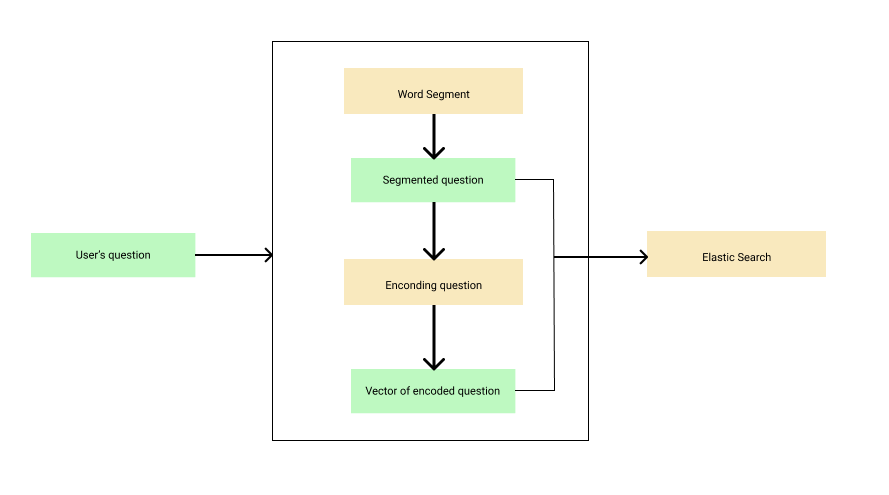
\includegraphics[width=\linewidth, height=7 cm]{images/elasticsearch_e}
\caption{Quy trình lưu dữ liệu xuống Elastic Search}
\label{fig:system2_s}
\end{figure*}

\pagebreak
\subsection{Phân loại từ trong câu hỏi}
Đầu tiên cần phải đề cập lại ở đây là có 3 cột dữ liệu đang có trong bộ dữ liệu đã được thu thập(dataset). Đó là cột câu hỏi, câu trả lời, ngày hỏi. Vì mục đích của hệ thống là hỏi đáp, đưa ra câu trả lời đúng và có mức độ liên quan gần nhất so với câu hỏi của người dùng nên đơn giản là chỉ ra được câu hỏi của người dùng nhập vào có bao nhiêu phần trăm là đồng nghĩa với câu hỏi có trong cơ sở dữ liệu. Vậy nên việc mã hoá dữ liệu cần phải làm là ở trên cột câu hỏi của dataset và câu hỏi của người dùng nhập vào từ giao diện website.

Trước khi mã hoá từ thì cần phải thực hiện một bước trước tiên đó là tách từ. Lý do cần phải thực hiện bước này trước tiên là vì tiếng việt là một ngôn ngữ không đơn giản, tiếng việt có tồn tại bên trong là các \textbf{từ ghép}. Vậy nên, nếu không thực hiện bước này trước tiên thì sẽ tạo ra một sự sai lệch về ngữ nghĩa trong khi mã hoá câu.

Ở đây thì nhóm sẽ thực hiện tách từ trong cột dữ liệu "Question" bằng PyVI như sau:

\begin{lstlisting}
	titles = [tokenize(doc["question"]) for doc in docs]
\end{lstlisting}

Dòng code này sẽ thực hiện công việc tách các từ ra, phân loại các từ đơn và từ ghép với nhau bằng dấu "$\_$".

\begin{figure*}[htp]
	\centering
	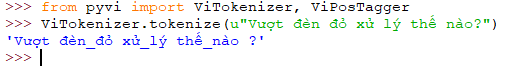
\includegraphics[scale=0.8]{images/tokenize}
	\caption{Tokenize một câu hỏi từ dataset}
	\label{fig:tokenize}
\end{figure*}

Khi thực hiện tách từ xong, biến dữ liệu \textbf{\textit{titles}} kiểu \textbf{str} sẽ lưu giữ tất cả các câu đã được tách từ. Theo như sơ đồ quy trình thì đây là thực hiện xong được bước Word Segment và được kết quả titles là Segmented question.
\pagebreak
\subsection{Mã hoá dữ liệu từ dataset}

Kết quả sau giai đoạn phân tách sẽ được hệ thống mã hóa, chuyển hóa thành các vector biểu diễn thông tin. Tại đây, nhóm áp dụng mô hình SimCSE cho tiếng Việt\cite{SimCSE_VNMESE} được phát triển dựa trên mô hình đào tạo sẵn là PhoBERT, với mục đích mã hóa, chuyển hóa thành các vector có thể biểu diễn đầy đủ ngữ nghĩa của từ của câu hỏi người dùng.\\

\begin{figure*}[htp]
	\centering
	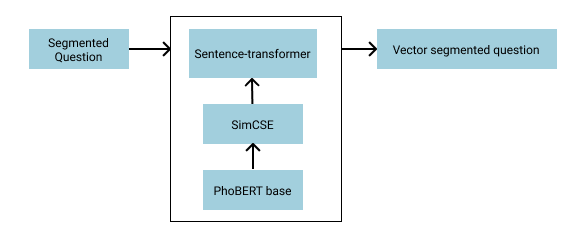
\includegraphics[scale=0.8]{images/encoding_graph}
	\caption{Quy trình thực hiện Encoding question}
\end{figure*}

Tại đây, dữ liệu đầu vào sẽ được chức năng Mã hóa thực hiện như sau:
\begin{itemize}
	\item Dữ liệu đầu vào sẽ được tính toán mã hóa dựa trên các từ, vị trí câu, vị trí từ trong câu với độ dài câu tối đa trong Position Embedding – mã hóa vị trí từ, là 512 tokens. 
	\item Token đầu tiên trong mỗi chuỗi đều có giá trị là [CLS], đại diện cho cả câu trong tác vụ phân loại. Token [SEP] dùng để phân biệt các câu với nhau.
	
	\begin{figure*}[htp]
		\centering
		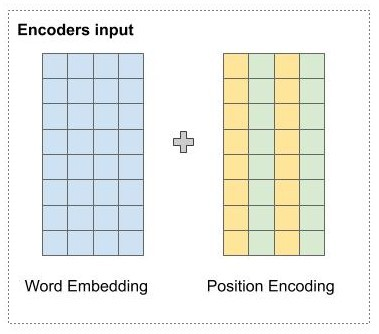
\includegraphics{images/position}
		\caption{Encoders Input}
		\label{fig:position}
	\end{figure*}
	\item Position Embedding – mã hóa vị trí từ trong câu: kiến trúc của BERT dựa trên kiến trúc của Transformers cho nên việc mã hóa vị trí từ trong câu cũng khá giống nhau. Vì Transformers có khả năng xử lý các từ song song nhưng nếu chỉ xử lý với mô hình Word Embedding sẽ không thể nào mô hình biết được vị trí của các từ để có thể hiểu ngữ nghĩa của câu. Vì vậy, cơ chế mã hóa vị trí từ trong câu xuất hiện để giải quyết vấn đề này bằng cách đưa thông tin vị trí của từ vào trong vector đại diện đầu vào.\\
\end{itemize}

Đối với việc mã hóa vị trí từ trong câu, PhoBERT hay BERT đều sử dụng công thức sau để tính toán vị trí\cite{TransformerModel}:

(PE)$_(pos,2i)$ = $\sin(pos/10000^{(2i/d_{model})})$

(PE)$_(pos,2i+1)$=$\cos(pos/10000^{(2i/d_{model})})$

Trong đó, pos là vị trí của từ trong câu, PE là giá trị phần tử thứ i trong ma trận Word Embedding có độ dài d$_{model}$.

Với việc mã hóa thành vector, SimCSE hay PhoBERT hay BERT đều dựa trên Transformers, sử dụng một cơ chế chung, cơ chế Attention., cho phép các từ khi được mã hóa sử dụng thông tin các từ liên quan đến nó.

Với mỗi từ, sẽ có ba vector tương ứng là Query, Key và Value. Các vector này được tính toán dựa trên ma trận Word Embedding.

Trong đó:
\begin{itemize}
	\item Query: vector đại diện, chứa thông tin của từ được tìm kiếm.
	\item Key: vector chứa thông tin của các từ được so sánh với vector Query.
	\item Value: vector chứa thông tin về nội dung, ý nghĩa của các từ trong vector Key.\\
\end{itemize}
Các bước tính toán attention vector có thể tóm lại bằng ba bước:

\begin{itemize}
	\item Bước 1: Tính ma trận Query, Key và Value dựa trên ma trận dữ liệu đầu vào là Word Embedding cộng với ma trận Position Embedding, tạo ra ba ma trận trọng số tương ứng với ba vector và nhân với ma trận dữ liệu đầu vào.
	\item Bước 2: Attetnion Score hay còn gọi là điểm tương quan hay trọng số, được tính bằng cách nhân hai ma trận Query và Key để so sánh mối liên hệ giữa các vector, cho ra được sự tương quan giữa chúng. Sau đó, dùng hàm Softmax để chuẩn hóa kết quả về đoạn [0-1] với ý nghĩa 1 là vector Query tương quan với vector Key, 0 là không có sự tương quan nào giữa chúng.
	\item Bước 3: Tính trọng số kết quả đầu ra bằng cách nhân ma trận kết quả Attention Score với ma trận Value để biểu diễn được thông tin của từ. \\	
\end{itemize}

\begin{figure*}[htp]
	\centering
	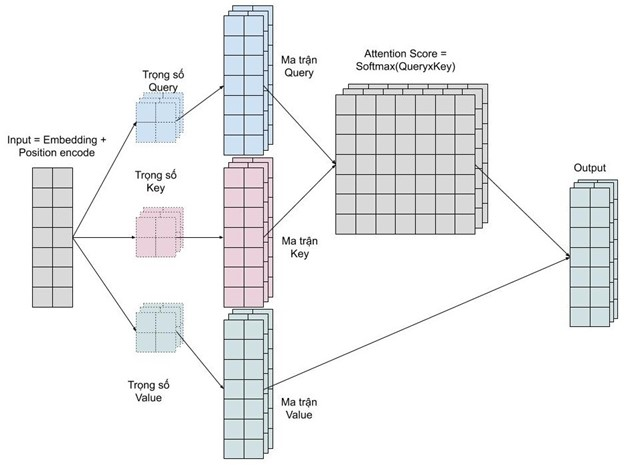
\includegraphics{images/matrix_encode}
	\caption{Ma trân mã hoá dữ liệu của BERT\cite{transformer}}
\end{figure*}

Trong thành phần Encoder của Transformers hay của BERT, thành phần Encoder bao gồm hai phần chính là Multi-Head Attention và Feedforward Network. Về bản chất, Multi-Head Attention là bao gồm nhiều lớp Self-Attention với cơ chế Attention đã được trình bày ở trên. Với mỗi Self-Attention sẽ cho ra được một mẫu kết quả khác nhau, nên việc sử dụng nhiều lớp Self-Attention sẽ giúp cho mô hình BERT cho ra kết quả chuẩn, có độ chính xác cao. Nó cho phép mô hình học được sự tương quan của từ dựa trên:
\begin{itemize}
	\item Từ kế trước của một từ
	\item Từ kế sau của một từ
	\item Những từ liên quan, tương đồng với một từ.
	
\end{itemize}

Lấy ví dụ người dùng nhập câu hỏi "Vượt đèn đỏ thì xử lý thế nào", sau khi phân tách thành các từ khóa "Vượt", "đèn\_đỏ", "xử\_lý", "thế\_nào", đưa vào mã hóa chuyển thành vector sẽ được nhận được ma trận vector của câu sau mã hóa với độ dài 768 tokens:

\begin{lstlisting}
[ 	1.9085e-01,  9.2255e-02, -8.8180e-02,  2.4886e-01, -1.8775e-02,
	...
	1.8846e-01,  3.8965e-02, 5.0931e-02,  6.2369e-02, -2.3854e-01]]
\end{lstlisting}

Cuối cùng, thực hiện xong quy trình mã hoá thì ta nhận được kết quả là Vector of encoded question như trên mô hình quy trình lưu dữ liệu xuống Elastic Search ở trên.

\subsection{Lưu dữ liệu đã mã hoá vào Elastic Search}

Sau khi có được 2 cột dữ liệu cần thiết là Segmented Question và Vector of encoded question, ta tiến hành thêm dữ liệu vào trong Elastic Search.

Đầu tiên, những giữ liệu chúng ta cần phải lưu lại trong Elastic Search cần có là:

\begin{table}[htp]
	\centering
	\begin{tabular}{|l|l|}
		\hline
		Tên thuộc tính & Kiểu dữ liệu \\ \hline
		ID             & text         \\ \hline
		Title          & text         \\ \hline
		Question       & text         \\ \hline
		Answer         & text         \\ \hline
		Title\_vector  & text         \\ \hline
	\end{tabular}
	\caption{Bảng kiểu dữ liệu thêm vào cơ sở dữ liệu}
	\label{tab:data-type-table}
\end{table}

\pagebreak
Để định danh các kiểu dữ liệu này trước khi lưu xuống cơ sở dữ liệu, ta cần một file để định danh cấu trúc của dữ liệu như sau:

\lstinputlisting[breaklines]{SourceCode/index.json}

Sau khi đã có file định danh cấu trúc cho dữ liệu, ta sử dụng thư viện Elasticsearch để bulk dữ liệu từ các biến lưu trữ thông tin về tách từ câu hỏi, vector tách từ câu hỏi vào trong Elastic Search.

Lý do để phải thêm 2 cột dữ liệu mới là vì trong khi tính toán độ tương đồng về ngữ nghĩa của câu thì cần phải so sánh với nhau ở dạng vector với nhau, từ đó mà đưa ra được kết quả chính xác hơn. 
\pagebreak
\subsection	{Kết quả}
Sau khi thêm dữ liệu thành công vào trong Elastic Search, để kiểm tra thông tin lưu trong Elastic Search thì ta thực hiện mở URL sau trên trình duyệt:

\begin{lstlisting}
	http://localhost:9200/demo_simcsejson/_search?pretty=true
\end{lstlisting}

Sau khi truy cập vào URL trên, Elastic Search sẽ trả về dữ liệu được lưu trữ trong có dạng như sau:

\begin{figure*}[htp]
\centering
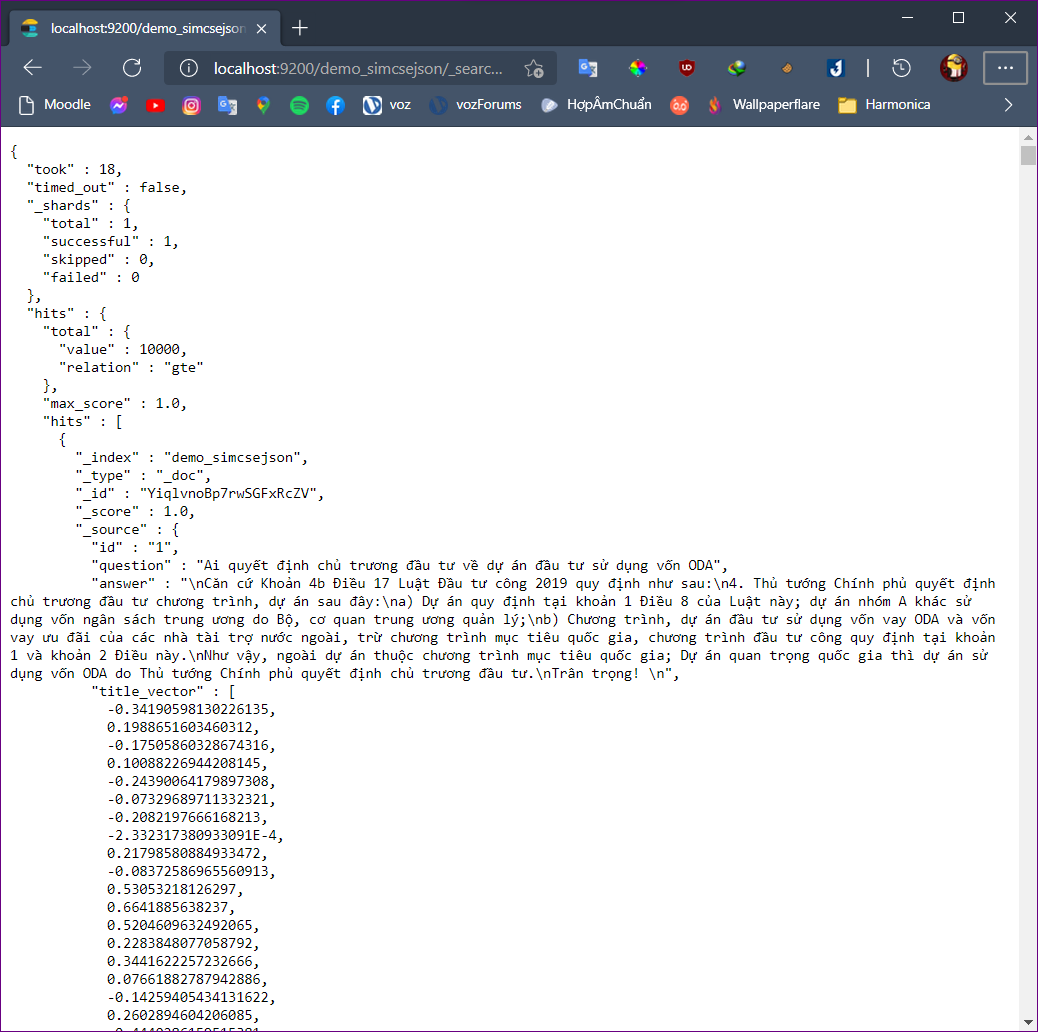
\includegraphics[width=\linewidth]{images/elastic_search_result}
\end{figure*}
\pagebreak
\section{Xử lý câu hỏi từ người dùng}
Ở mục này, câu hỏi sẽ được người dùng nhập vào trong hệ thống và được hệ thống xử lý tìm kiếm bằng cách so sánh mức độ tương đồng về ngữ nghĩa thông qua việc mã hoá câu hỏi của người dùng nhập vào thành vector câu hỏi rồi so sánh với các vector câu hỏi có trong cơ sở dữ liệu.

\begin{figure*}[htp]
\centering
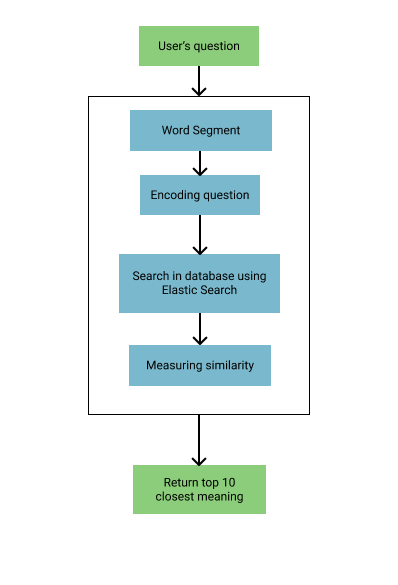
\includegraphics[width=12 cm]{images/asking}
\caption{Quy trình xử lý câu hỏi từ người dùng}
\label{fig:asking}
\end{figure*}
\pagebreak
Câu hỏi của người dùng sau khi nhập vào từ giao diện website sẽ được gửi từ web server đến phía Back-end của hệ thống. Khi nhận được dữ liệu câu hỏi, hệ thống sẽ bắt đầu thực hiện xử lý câu hỏi của người dùng theo từng bước là:
\begin{itemize}
	\item Tách từ trong câu
	\item Mã hoá câu đã được tách từ
	\item Tìm kiếm trong cơ sở dữ liệu vector giống với vector câu hỏi nhất
	\item So sánh mức độ tương đồng với câu hỏi
	\item Trả về những câu hỏi có mức độ tương đồng ngữ nghĩa với câu hỏi của người dùng cao nhất
\end{itemize}
\subsection{Tính toán mức độ tương đồng ngữ nghĩa giữa các câu}
Ở mục này, nhóm sẽ giải quyết bài toán được đặt ra từ trước để có thể tiến hành hoàn thành hệ thống là bài toán tính mức độ tương đồng ngữ nghĩa giữa các câu.

Sau quá trình tìm hiểu các phương pháp được giới thiệu để tính toán được mức độ tương đồng giữa các vector với nhau, các phương pháp đều quy về một hướng đó là so sánh khoảng các giữa các vector với nhau. Có 3 phương pháp so sánh vector với nhau mà được Google giới thiệu trong khoá học\cite{MeasureSimilarityGoogle} là:

\begin{itemize}
	\item Euclidean distance: Khoảng cách Euclide giữa hai vector
	\item Cosine: Góc giữa hai vector
	\item Dot Product: Tích vô hướng giữa hai vector
\end{itemize}

Xét riêng tích vô hướng giữa hai vector và góc giữa hai vector, chúng sẽ là giống nhau khi độ dài hai vector cùng bằng nhau và bằng 1. Nhưng nếu độ dài của hai vector không bằng 1 thì việc tính toán bằng tích vô hướng giữa các vector sẽ trở nên phức tạp hơn so với khi sử dụng góc giữa các vector. Vậy nên nếu phải chọn phương pháp nào giữa tích vô hướng và góc giữa các vector thì sử dụng góc giữa các vector sẽ là sự lựa chọn tốt hơn.

Bên cạnh đó, việc sử dụng khoảng cách Euclide trong không gian nhiều chiều sẽ được tính theo công thức là:
\begin{figure*}[htp]
\centering
$d\left( p,q\right)   = \sqrt {\sum _{i=1}^{n}  \left( q_{i}-p_{i}\right)^2 }$
\end{figure*}

Nhìn vào công thức tính góc giữa các vector là:

\begin{figure*}[htp]
	\centering
$\text{similarity}=\cos(\theta )={\mathbf {A} \cdot \mathbf {B}  \over \|\mathbf {A} \|\|\mathbf {B} \|}={\frac {\sum \limits _{i=1}^{n}{A_{i}B_{i}}}{{\sqrt {\sum \limits _{i=1}^{n}{A_{i}^{2}}}}{\sqrt {\sum \limits _{i=1}^{n}{B_{i}^{2}}}}}} $
\end{figure*}

Nếu xét trên không gian nhiều chiều, ta sẽ thấy được rằng công thức giữa Euclide distance và Cosine Distance cũng sẽ đưa về một điểm chung đó là góc giữa hai vector. Vậy nên, sử dụng Cosine Distance sẽ là sự lựa chọn thích hợp trong trường hợp này. Ngoài ra, khi sử dụng chung với Elastic Search thì sẽ được Elastic Search hỗ trợ hàm được xây dựng sẵn trong việc tính toán.

Với Ai và Bi là thành phần của vector A và B tương ứng. Giá trị của cosine luôn nằm trong đoạn [-1,1]:
\begin{itemize}
	\item Giá trị cosine bằng 1, hai vector trùng nhau, suy ra, A và B giống nhau.
	\item Giá trị cosine càng tiến về -1, nghĩa là A và B khác nhau.
\end{itemize}

Như vây, nếu giá trị cosine giữa hai vector càng tiến về 1, hai vector càng có sự tương đồng với nhau. Áp dụng vào hệ thống, ta suy ra được, nếu giá trị cosine giữa vector đại diện câu hỏi của người dùng và vector đại diện câu hỏi trong bộ dữ liệu càng gần 1, thì nội dung hai câu hỏi càng tương đồng.

Nhóm em đã tiến hành tìm kiếm sự tương đồng giữa vector đại diện câu hỏi người dùng và vector đại diện câu hỏi trong bộ dữ liệu bằng cách truyền vector đại diện câu hỏi người dùng vào Elastic Search, tính độ tương đồng Cosine Similarity nhờ vào hàm chức năng của Elastic Search. Cosine Similarity trên Elastic Search sau khi tính toán sẽ cộng thêm 1 để tránh giá trị âm, như vậy giá trị cosine nằm trong [1,2]. Về mặt ý nghĩa không khác gì giá trị cosine nằm trong [-1,1]. Chúng em thu được một số kết quả như sau:


\subsection {Trả về kết quả sau khi so sánh}
Vì Elastic Search có hỗ trợ trong việc tính toán Cosine Distance, vậy nên trong khi tìm kiếm dữ liệu bằng Elastic Search, ngoài điều việc tìm kiếm các tách từ giống nhau thì ta chèn thêm một điều kiện nữa là có Cosine Distance nhỏ nhất.

Sau đây là đoạn script dùng để search dữ liệu trong Elastic Search:
\begin{lstlisting}
 	"script_score": {
		"query": {
			"match_all": {}
		},
		"script": {
			"source": "cosineSimilarity(params.query_vector, 'title_vector') + 1.0",
			"params": {"query_vector": query_vector}
		}
	}
\end{lstlisting}

Khi nhìn vào đoạn script trên, query\_vector là câu hỏi của người dùng nhập vào được tách từ(Word Segment) và cosineSimilarity là điều kiện search khi ánh xạ qua so với Query search của cơ sở dữ liệu quan hệ.
 

Câu hỏi của người dùng: “Vượt đèn đỏ thì xử lý thế nào”.
\begin{itemize}
	\item Vector đại diện cho “Mức phạt hành vi vượt đèn đỏ” cho giá trị độ tương đồng bằng 1.8454137.
	\item Vector đại diện cho “Phạt bao nhiêu nếu ô tô vượt đèn đỏ” cho giá trị độ tương đồng bằng 1.7503384
	\item Vector đại diện cho “Hành vi điều khiển xe máy mà vượt đèn đỏ sẽ bị xử phạt bao nhiêu” cho giá trị độ tương đồng bằng 1.7825083.
	\item Vector đại diện cho “Sử dụng biển quảng cáo che mất đèn đỏ giao thông xử phạt thế nào” cho giá trị độ tương đồng 1.7325894.
\end{itemize}

Sau khi đã lấy ra được tập câu hỏi và trả lời thoả mãn được yêu cầu của hệ thống thì cần phải trả về kết quả ra để phía web server có thể lấy được kết quả trả về để gửi lại phía bên phía Front-end, hiển thị kết quả cho người dùng.


\chapter{Kết quả}
\label{Chapter5}

\textit{Nội dung chương này sẽ trình bày về các kết quả mà nhóm đã đạt được trong quá trình giải quyết các bài toán con để hoàn thành đồ án.}

\section{Kết quả của quy trình thu thập dữ liệu}
Sau khi thực hiện xong việc Scraping data, kết quả thu được là \textbf{232321} cặp câu hỏi và câu trả lời, có ngày tháng được hỏi ở hai định dạng dữ liệu là CSV và JSON.

Dữ liệu ban đầu thu thập về là ở định dạng file CSV nhưng vì lý do cần phải xử lý định dạng lại cấu trúc hiển thị dữ liệu trên website nên nhóm đã chuyển đổi định dạng của file CSV sang file JSON. 

Qua đó, nhóm đã giải quyết xong được bài toán đầu tiên cần phải giải quyết trong các bàn toán nhỏ cần phải giải để có hoàn thành được hệ thống.

\section{Kết quả sau khi mã hoá dữ liệu câu hỏi sau khi thu thập và lưu vào Elasticsearch}
Sau khi thêm dữ liệu thành công vào trong Elastic Search, để kiểm tra thông tin lưu trong Elastic Search thì ta thực hiện mở URL sau trên trình duyệt:

\begin{lstlisting}
	http://localhost:9200/demo_simcsejson/_search?pretty=true
\end{lstlisting}

Sau khi truy cập vào URL trên, Elastic Search sẽ trả về dữ liệu được lưu trữ trong có dạng như sau:

\begin{figure*}[htp]
\centering
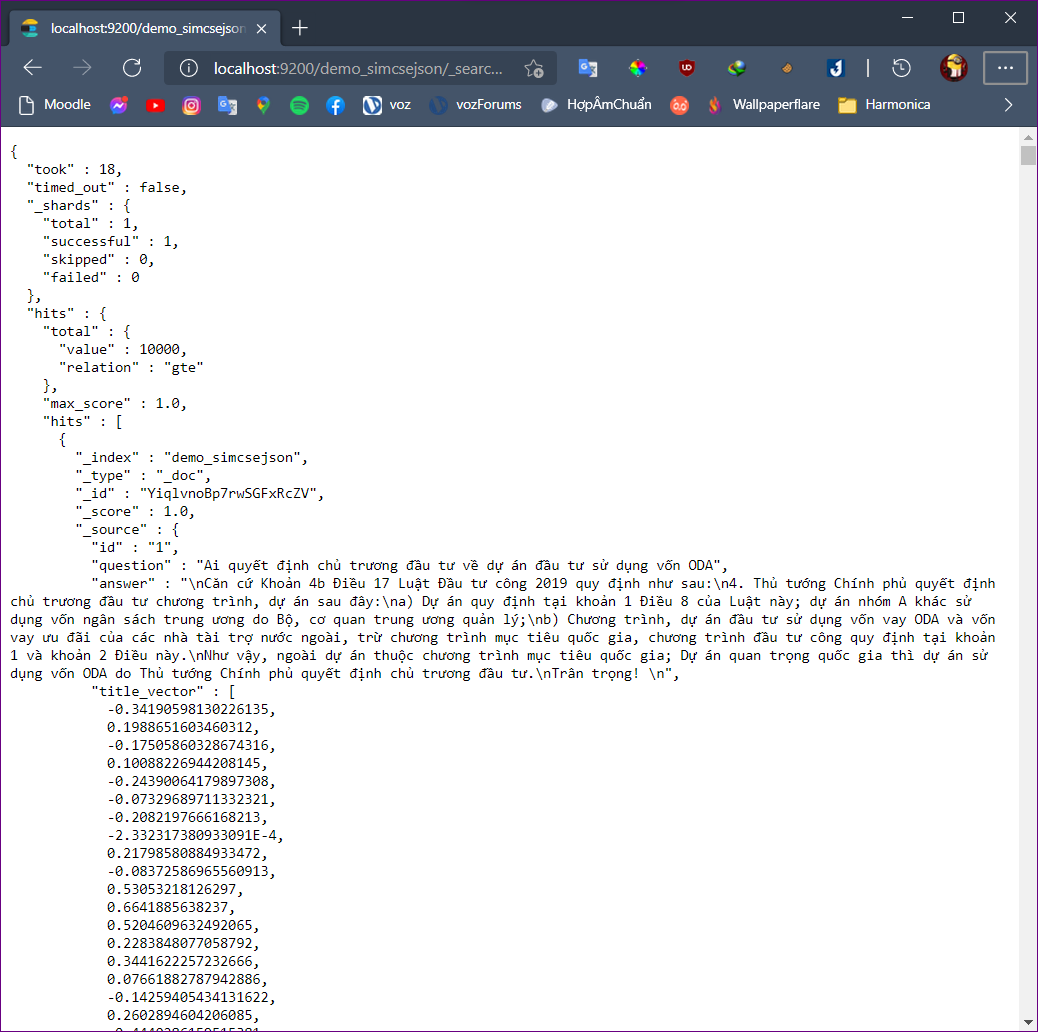
\includegraphics[width=\linewidth]{images/elastic_search_result}
\caption{Dữ liệu được lưu vào trong Elasticsearch sau khi Encode.}
\label{fig:elastic_search_result}
\end{figure*}
\pagebreak

Những mục cần lưu ý trong dữ liệu được tô đỏ trong hình ảnh trên chính là những cột dữ liệu được lưu trữ trong Elasticsearch. Những thuộc tính đã được nhấn mạnh là cần lưu trữ đã được nêu ở chương 4 là những thuộc tính nằm trong phần được đánh dấu đỏ.

Qua nội dung này thì nhóm đã hoàn thành được việc giải bài toán mã hoá văn bản tiếng việt và xử lý ngôn ngữ tự nhiên.
\section{Kết quả của quy trình nhận dữ liệu từ Back-end và hiển thị lên Front-end}

Sau khi đã lấy ra được tập câu hỏi và trả lời thoả mãn được yêu cầu của hệ thống thì cần phải trả về kết quả ra để phía web server có thể lấy được kết quả trả về để gửi lại phía bên phía Front-end, hiển thị kết quả cho người dùng.

Respond dữ liệu từ Back End lên Front End:

Template Engine: jinja2

Với việc sử dụng jinja2 là một template engine, ta có thể hiển thị dễ dàng các biến results và raw\_text đã được truyền vào trước đó bởi hàm render\_template bằng cách gọi trực tiếp trong các HTML template:

\begin{lstlisting}
	<p class="input" style="...">Cau hoi da nhap: "{{raw\_text}}"</p>
	<p class="input" style="...">{{results[0][1]}}</p>
\end{lstlisting}

Kết quả nhận được là: 
\begin{figure*}[htp]
	\centering
	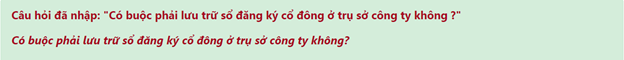
\includegraphics{images/res1}
	\caption{Kết quả của render template.}
	\label{fig:res1}
\end{figure*}

Jinja2 còn có thể dùng để viết ra các hàm để xử lý dữ liệu được đổ vào Website:

\begin{lstlisting}
	{% if results != null %}
		{{answer(answer=results[0][2])}}
		{% endif %}		
		\end{lstlisting}
		
		Kết quả nhận được là: 
		
		\begin{figure*}[htp]
			\centering
			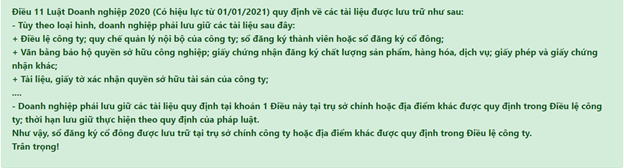
\includegraphics{images/res2}
			\caption{Kết quả nhận được khi sử dụng Jinja2.}
			\label{fig:res2}
		\end{figure*}
		
		
		\begin{lstlisting}
			{% for para in results if para[0] != 1 %}
				{{group_QA(data_id = para[0] - 1,
						question = para[1],
						answer = para[2])}}
				{% endfor %
				\end{lstlisting}
				
				Kết quả nhận được là: 
				
				\begin{figure*}[htp]
					\centering
					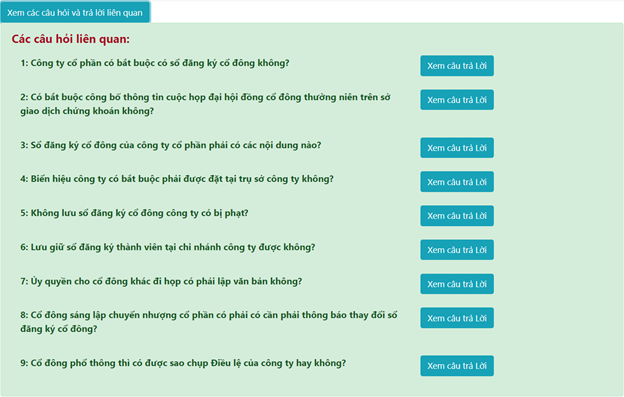
\includegraphics[scale=0.8]{images/final}
					\caption{Kết quả nhận được khi nhấn vào button "Xem câu hỏi liên quan".}
					\label{fig:final}
				\end{figure*}
\section{Tính đúng đắn của mô hình sau khi đánh giá thủ công}

Cuối cùng, để đánh giá được mô hình sử dụng trong đồ án có độ chính xác là bao nhiêu, nhóm thực hiện đánh giá thủ công trên 100 câu hỏi. Đánh giá mô hình được dựa trên so sánh độ chính xác của kết quả trả về đầu tiên (là kết quả được trả về với độ chính xác cao nhất từ hệ thống) của 3 phương pháp là:
\begin{itemize}
	\item [-] Phương pháp tìm kiếm bằng từ khoá của Elasticsearch.
	\item [-] Phương pháp tìm kiếm bằng mô hình áp dụng Pre-trained SimCSE.
	\item [-] Phương pháp tìm kiếm bằng mô hình sử dụng Pre-trained SimCSE và được sắp xếp lại bằng mô hình tự xây dựng trên dữ liệu STS và dữ liệu Pháp luật gán nhãn thủ công.
\end{itemize}

Kết quả trả về của từng phương pháp được tính như sau:
\begin{itemize}
	\item Phương pháp tìm kiếm bằng từ khoá của Elasticsearch: Kết quả được trả về là kết quả có \textit{\_score} cao nhất. Công thức tính được \textit{\_score} được Elasticsearch giải thích là:
	\begin{center}
	$IDF score * TF score * fieldNorms$\\
	\end{center}

	Trong đó, TF score là tần suất xuất hiện của term trong field. Càng xuất hiện nhiều, relevance càng cao. Term frequency (tf) của t trong document d được tính bằng căn bậc hai của số lần t xuất hiện trong d. Vậy nên ta sẽ có công thức để tính TF score là: $tf(t, d) = \sqrt{frequency}$\\
	IDF score là đánh giá tần suất xuất hiện của term trên toàn bộ index, càng xuất hiện nhiều, càng ít thích hợp. IDF score được tính theo công thức là: $idf(t) = 1 + \log{\frac{numDocs} {docFreq+1}}$\\
	fieldNorms là đánh giá độ dài của field. Field càng ngắn, thì term sẽ có giá trị càng cao; và ngược lại. fieldNorms sẽ được tính theo công thức là: $norm(d) =\frac{1}{\sqrt{numTerms}}$\\
	Các giá trị này sẽ được Elasticsearch hỗ trợ tính toán.
	\item Phương pháp sử dụng Pre-trained SimCSE: Kết quả trả là góc nhỏ nhất giữa vector câu hỏi của người dùng và vector câu hỏi có trong cơ sở dữ liệu.
	\item Phương pháp sử dụng Pre-trained SimCSE kết hợp với mô hình xây dựng trên bộ dữ liệu STS và Pháp luật thì ngoài kết quả là góc của vector thì còn có khoảng cách Euclide giữa các vector đấy là nhỏ nhất.
\end{itemize}

Sau khi chọn ra được câu hỏi đầu tiên từ hệ thống thông qua 3 phương pháp được nêu trên, nhóm có bảng kết quả thực hiện đánh giá như sau:
\begin{itemize}
	\item L1 là khi sử dụng bằng cách tìm kiếm từ khoá sử dụng Elasticsearch 
	\item L2 là khi tìm kiếm bằng mô hình áp dụng Pre-trained SimCSE
	\item L3 là khi tìm kiếm bằng mô hình sử dụng Pre-trained SimCSE và được sắp xếp lại bằng mô hình tự xây dựng trên dữ liệu STS và dữ liệu Pháp luật gán nhãn thủ công.
	\item C1 là số lượng câu hỏi được đánh giá có liên quan đến câu hỏi đầu vào ở website hoidap.thuvienphapluat.vn.
	\item C2 là số lượng câu hỏi được đánh giá có liên quan đến câu hỏi đầu vào ở Hệ thống Hỏi đáp Pháp luật Việt Nam.
	
\end{itemize}

\pagebreak

\begin{longtable}{|>{\hspace{0pt}}m{0.038\linewidth}|>{\hspace{0pt}}m{0.531\linewidth}|>{\hspace{0pt}}m{0.038\linewidth}|>{\hspace{0pt}}m{0.038\linewidth}|>{\hspace{0pt}}m{0.038\linewidth}|>{\hspace{0pt}}m{0.04\linewidth}|>{\hspace{0pt}}m{0.042\linewidth}|}
	\caption{Bảng rút gọn 100 câu hỏi dùng để kiểm tra độ chính xác của model}\\ 
	\hline
	\textbf{ID} & \textbf{Question} & \textbf{L1} & \textbf{L2} & \textbf{L3} & \textbf{C1} & \textbf{C2} \endfirsthead 
	\hline
	1 & Bán hàng rong có phải đăng ký kinh doanh không ? & 1 & 1 & 1 & 1 & 8 \\ 
	\hline
	2 & Điều kiện hưởng lương hưu của sĩ quan, quân nhân & 1 & 1 & 1 & 1 & 6 \\ 
	\hline
	3 & Thời hạn sang tên sổ đỏ khi mua bán đất & 0 & 0 & 1 & 2 & 10 \\ 
	\hline
	4 & Điều kiện mang thai hộ vì mục đích nhân đạo & 0 & 1 & 1 & 8 & 10 \\ 
	\hline
	5 & Có được khai sinh là ngày âm lịch không? & 0 & 0 & 0 & 2 & 1 \\ 
	\hline
	6 & Lương và chế độ việc làm của phụ nữ trong thời gian nuôi con nhỏ? & 0 & 1 & 0 & 0 & 8 \\ 
	\hline
	7 & Mức phạt bán buôn thuốc lá không rõ nguồn gốc xuất xứ? & 0 & 1 & 1 & 1 & 10 \\ 
	\hline
	8 & Không lập biên bản có được tạm giữ xe không? & 1 & 1 & 1 & 2 & 9 \\ 
	\hline
	9 & Mức phạt khi vi phạm về sử dụng lao động chưa thành niên & 0 & 1 & 0 & 0 & 7 \\ 
	\hline
	10 & Bảo đảm dự thầu áp dụng trong trường hợp nào? & 1 & 1 & 1 & 2 & 8 \\ 
	\hline
	11 & Quy trình đấu thầu lại sau khi hủy thầu như thế nào? & 0 & 0 & 0 & 0 & 5 \\ 
	\hline
	12 & Thời gian nộp, thời gian hoàn trả bảo đảm thực hiện hợp đồng & 0 & 0 & 0 & 2 & 6 \\ 
	\hline
	13 & Hỏi về thời điểm đóng thầu & 0 & 0 & 0 & 0 & 5 \\ 
	\hline
	14 & Có được bổ sung nhà thầu liên danh? & 0 & 1 & 1 & 1 & 6 \\ 
	\hline
	15 & So sánh đầu tư trực tiếp nước ngoài và đầu tư gián tiếp nước ngoài & 0 & 0 & 0 & 1 & 9 \\ 
	\hline
	16 & Thủ tục chuyển nhượng dự án đầu tư cho nhà đầu tư nước ngoài & 1 & 1 & 1 & 7 & 7 \\ 
	\hline
	17 & Thành lập chi nhánh công ty có vốn đầu tư nước ngoài cần làm gì? & 0 & 0 & 1 & 4 & 5 \\ 
	\hline
	18 & Độ tuổi được lập di chúc?~ & 0 & 1 & 1 & 1 & 7 \\ 
	\hline
	19 & Dưới 18 tuổi có được phép lập di chúc không? & 1 & 1 & 0 & 0 & 10 \\ 
	\hline
	20 & Nếu có nhiều di chúc ở nhiều thời điểm khác nhau, di chúc nào có hiệu lực? & 1 & 1 & 1 & 4 & 7 \\ 
	\hline
	21 & Các trường hợp nào cháu được hưởng di sản thừa kế của ông bà? & 0 & 1 & 1 & 2 & 10 \\ 
	\hline
	22 & Con riêng có được hưởng thừa kế? & 1 & 1 & 1 & 6 & 10 \\ 
	\hline
	23 & Không thực hiện nghĩa vụ phụng dưỡng cha mẹ có được hưởng thừa kế? & 1 & 1 & 1 & 0 & 2 \\ 
	\hline
	24 & Tiền phúng viếng là tài sản của ai? & 0 & 0 & 1 & 0 & 8 \\ 
	\hline
	25 & Người đã chết có được hưởng di sản thừa kế không? & 0 & 1 & 1 & 0 & 8 \\ 
	\hline
	26 & Quy định về phân chia di sản thừa kế theo pháp luật mới nhất & 1 & 0 & 1 & 2 & 9 \\ 
	\hline
	27 & Điều kiện có hiệu lực của di chúc bằng miệng? & 1 & 1 & 1 & 3 & 9 \\ 
	\hline
	28 & Chưa có giấy chứng nhận quyền sử dụng đất chia thừa kế được không? & 0 & 1 & 1 & 0 & 8 \\ 
	\hline
	29 & Đánh bạc nhiều lần bị phạt thế nào? & 0 & 0 & 0 & 2 & 10 \\ 
	\hline
	30 & Xử phạt khi sử dụng ma túy lần đầu? & 0 & 1 & 0 & 0 & 5 \\
	\hline
\end{longtable}

\pagebreak

Qua bảng kết quả đánh giá trên thì nhóm có công thức để đánh giá kết quả tìm kiếm bằng 3 phương pháp trên là:

\begin{center}
	$result = \frac{\sum_{t=1}^{N}(L_{i}(1))}{N}$    
\end{center}

Với 
\begin{itemize}
	\item \textbf{$\sum_{t=1}^{N}(L_{i}(1))$} là tổng số các giá trị bằng 1 có trong bảng đánh giá của cột kết quả đánh giá L1, L2, L3
	\item \textbf{N} là tổng số câu hỏi được đem ra làm mẫu để đánh giá các phương pháp, ở đây N có giá trị là 100.
\end{itemize}

\begin{center}
	$result' = \frac{\sum_{t=1}^{N}(C_{i}(1))}{N*10}$    
\end{center}
\begin{itemize}
	\item $C_{i}$  là số lượng câu hỏi được đánh giá có liên quan đến câu hỏi đầu vào.
	\item $N$ là tổng số câu hỏi được test, $N$=100.
	
\end{itemize}
Kết quả trả về đầu tiên mà hệ thống trả về sẽ được các thành viên đánh giá thủ công. Kết quả nào được thành viên kiểm thử đánh giá là đúng so với câu hỏi người dùng thì sẽ có giá trị là \textbf{1} và ngược lại.

\begin{itemize}
	\item Phương pháp tìm kiếm bằng Elasticsearch: 43\%
	\item Phương pháp tìm kiếm bằng mô hình Pre-trained SimCSE: 74\%
	\item Phương pháp tìm kiếm bằng mô hình Pre-trained SimCSE kết hợp với mô hình xây dựng trên dữ liệu Luật pháp: 49\%
	\item Hệ thống website hoidap.thuvienphapluat.vn: 8.2\% 
	\item Hệ thống Hỏi đáp Pháp luật Việt Nam: 74\% 
	
\end{itemize}

Qua kết quả đánh giá, mặc dù Elasticsearch rất có danh tiếng trong khả năng tìm kiếm dữ liệu với độ chính xác cao và nhanh chóng, nhưng khi áp dụng trí tuệ nhân tạo vào trong bài toán tìm kiếm thì độ chính xác của việc tìm kiếm đã được cải thiện tới 31\%. Bên cạnh đó, việc đào tạo trên dữ liệu Pháp luật với khối lượng dữ liệu Pháp luật nhỏ(chỉ 400 dòng dữ liệu) đã có cải thiện hơn 6\% so với khi chỉ sử dụng tìm kiếm bằng từ khoá thông thường. Vậy nên, nếu như mô hình được đào tạo và xây dựng lại với khối lượng dữ liệu nhiều hơn thì việc nâng cao độ chính xác của mô hình lên là việc chắc chắn sẽ xảy ra. 

\chapter{Kết luận}
\label{Chapter6}

\textit{Chương 6 sẽ trình bày những kết quả đạt được sau khi hoàn thành xong đề tài đồ án này, định hướng phát triển của ứng dụng trong tương lai.}

\section{Kết quả đạt được}

Xuyên suốt quá trình thực hiện đồ án tốt nghiệp trong 6 tháng qua, nhóm đã học tập và tích luỹ được rất nhiều kiến thức tuy rằng không được đào tạo trong chuyên ngành nhưng rất bổ ích cho việc trau dồi kiến thức về ngành Công Nghệ Thông Tin.

\subsection{Về mặt kiến thức}
\begin{itemize}
	\item [-] Tìm hiểu và áp dụng thành công kĩ thuật Scraping Web để thu thập dữ liệu từ các web site.
	\item [-] Nghiên cứu các thư viện tách từ theo các từ ghép như underthesea, VnCoreNLP, python vietnamese toolkit.
	\item [-] Tìm hiểu và áp dụng được pre-trained Pho BERT, ngoài ra còn tự build được một mô hình của riêng nhóm trên dữ liệu tự tạo.
	\item [-] Sử dụng được Elastic Search để xử lý chính cho hệ thống.
	\item [-] Xây dựng được Web Server cho hệ thống.
	\item [-] Giải quyết được tất cả các bài toán cần phải giải quyết để xây dựng hệ thống.
\end{itemize}

\subsection{Về mặt ứng dụng}

Nhóm đã có thử đưa ứng dụng lên một máy chủ VPS Azure để có thể host ứng dụng thành một ứng dụng Web hoàn chỉnh nhưng vì lý do chi phí để mở máy chủ quá cao và chưa thành công trong việc đăng kí tên miền cho máy chủ nên hiện về mặt ứng dụng thì vẫn chưa thành công. Nhóm có thử sử dụng qua các dịch vụ miễn phí hoặc là có ưu đãi cho sinh viên nhưng vẫn không thể đáp ứng được việc đủ bộ nhớ để lưu dữ liệu Elasticsearch và các thư viện của hệ thống, bộ nhớ Ram phục vụ cho Elasticsearch hoạt động.
\section{Định hướng phát triển}

Vì giới hạn về kĩ năng cũng như thời gian, hiện tại nhóm đã hoàn thành tốt nhất sản phẩm cho hiện tại nhưng vẫn còn một số hạn chế. Trong tương lai, nhóm sẽ phát triển một số tính năng sau nữa để có thể hoàn thành nhất sản phẩm ví dụ như:
\begin{itemize}
	\item [-] Xây dựng thêm tính năng thêm số lượng câu hỏi và câu trả lời vào hệ thống, vì hiện tại hệ thống chỉ sử dụng trên dữ liệu được lưu trữ sẵn trong cơ sở dữ liệu và không thể thêm dữ liệu mới vào vậy nên khi cần thêm mới bộ câu hỏi và câu trả lời thì nhóm cần phải xây dựng thêm tính năng mới để có thể thêm mới dữ liệu vào được.
	\item [-] Nâng cấp được độ chính xác của mô hình đào tạo trên dữ liệu Pháp luật. Hiện tại thì mô hình vẫn chỉ dừng lại ở mức độ là kiểm tra câu hỏi của người dùng có tương đồng với dữ liệu có trong cơ sở dữ liệu hay không chứ chưa thể kiểm tra được câu hỏi của người dùng đồng nghĩa hay trái nghĩa với câu hỏi được lưu trữ trong cơ sở dữ liệu. Vậy nên, định hướng để đưa mô hình đạo tạo chính xác hơn thì nhóm cần phải thực hiện được chức năng này.
	\item [-] Triển khai được hệ thống hoạt động như Web app hoàn chỉnh. Hiện tại vì lý do kinh phí duy trì được lượng dữ liệu trong cơ sở dữ liệu và sử dụng Elasticsearch để tìm kiếm cũng như có đủ phần cứng để chạy được mô hình pre-trained PhoBERT thì cần phải có một phần cứng đủ mạng để có thể chịu được hệ thống. Nhưng do kinh phí để có thể duy trì được một hệ thống như vậy tương đối lớn so với nhóm và cũng như nhóm thể làm kịp được việc triển khai hệ thống nên phần này nhóm sẽ định hướng để phát triển thêm.
\end{itemize}




% Công trình của tác giả (nếu không có thì comment 02 dòng dưới)
%\addcontentsline{toc}{chapter}{Danh mục công trình của tác giả}
%\include{Appendix/publish}

% In tài liệu tham khảo
\addcontentsline{toc}{chapter}{Tài liệu tham khảo}
\printbibheading[title={Tài liệu tham khảo}]

\printbibliography[heading=subbibliography, title={Tiếng Việt}, keyword=Viet, resetnumbers=true]

\DeclareNameAlias{sortname}{last-first}
\DeclareNameAlias{default}{last-first}

\printbibliography[heading=subbibliography, title={Tiếng Anh}, notkeyword=Viet, resetnumbers=4] 



% ===================================================================== %
% CHÚ Ý: phải gán lại resetnumbers=số tài liệu tham khảo tiếng Việt + 1 %
% ===================================================================== %


\end{document} 